% =====================================================================
%DIF LATEXDIFF DIFFERENCE FILE
%DIF DEL _old_tmp.tex   Wed Nov 18 01:18:27 2026
%DIF ADD _new_tmp.tex   Wed Nov 18 01:18:27 2026
%DIF 2-3c2
%DIF < % Fully Symmetry-Conditioned Rigid-Body Flow Matching for
%DIF < % Molecular-Crystal Structure Prediction
%DIF -------
% ACS Omega resubmission (ao-2026-09173w) -- REBUILT AROUND THE N3 BENCHMARK, draft 2026-11-17 %DIF > 
%DIF -------
%
%DIF 5-7c4-5
%DIF < % ACS Omega, CODEN acsodf. Transferred from J. Chem. Inf. Model.
%DIF < % ACS `achemso` class (manuscript=article). Bibliography style is owned by
%DIF < % achemso -- do NOT add \bibliographystyle or load natbib.
%DIF -------
% ACS `achemso` class (manuscript=article). Bibliography style is owned by achemso -- do NOT add %DIF > 
% \bibliographystyle or load natbib. ACS Omega places Methods AFTER Conclusions. %DIF > 
%DIF -------
%
%DIF 9-17c7-12
%DIF < % STRUCTURE NOTE (differs from the JCIM package): ACS Omega places Methods
%DIF < % AFTER Conclusions. The orientation decomposition, which is an empirical
%DIF < % finding rather than a procedure, is promoted into Results and Discussion;
%DIF < % the procedural material moves to the Methods section at the back.
%DIF < %
%DIF < % Numbers: Phase B (e035b8d), E1 (581723c), E3 (1224870), E2 scale (ce0e5d0),
%DIF < % E4 bench (phaseE4), Phase F ladder (FINDINGS_F_FINAL.md, phaseF3{a..f}).
%DIF < % Extended methods (family mask, finisher) live in the Supporting Information
%DIF < % (paper/submissions/ACSOmega/si.tex).
%DIF -------
% EVERY N3 NUMBER comes from generated/*.tex, written by scripts/n3_paper_numbers.py from %DIF > 
% results/n3/n3_results.json (committed f1c713a, before interpretation). Never type a result by hand. %DIF > 
% CLAIM RULES: tasks/n3_protocol.md section 4 (outcome -> claim map), section 5 (frozen Table R %DIF > 
% wording) and section 6 (abstract rules). Forbidden: any CSP/end-to-end claim for OURS; "better than %DIF > 
% physics-based search"; any representability claim against MolCrystalFlow's per-copy representation. %DIF > 
% The pre-N3 version is archived in archive/main-archive-2026-11-17-pre-N3.tex. %DIF > 
%DIF -------
% =====================================================================
\documentclass[journal=acsodf,manuscript=article]{achemso}

%DIF 21c16-18
%DIF < \usepackage{amsmath,amssymb}
%DIF -------
\usepackage{amsmath} %DIF > 
\usepackage[T1]{fontenc} %DIF > 
\usepackage{newtxtext,newtxmath} % Times text and math (ACS house style); newtxmath supplies the amssymb symbols %DIF > 
%DIF -------
\usepackage{graphicx}
\usepackage{booktabs}
%DIF 24a21-22
\usepackage{xcolor} %DIF > 
\usepackage{rotating} %DIF > 
%DIF -------
\graphicspath{{figures/}{../../figures/}}

%DIF 26a25-113
% GENERATED by scripts/n3_paper_numbers.py from results/n3/n3_results.json and results/n3/table_r_testB.json -- do not edit %DIF > 
\newcommand{\nN}{1{,}000} %DIF > 
\newcommand{\nOursPick}{8.47} %DIF > 
\newcommand{\nOursSd}{1.35} %DIF > 
\newcommand{\nOursSeeds}{8.5, 7.1, 9.8} %DIF > 
\newcommand{\nOursDraw}{0.98} %DIF > 
\newcommand{\nOursAny}{13.6} %DIF > 
\newcommand{\nOursSec}{16.8} %DIF > 
\newcommand{\nOursNtwoPick}{6.47} %DIF > 
\newcommand{\nOursNtwoSd}{0.32} %DIF > 
\newcommand{\nSearchPick}{99.4} %DIF > 
\newcommand{\nIEPick}{58.9} %DIF > 
\newcommand{\nMcfRPick}{0.00} %DIF > 
\newcommand{\nMcfRGPick}{0.13} %DIF > 
\newcommand{\nIvPPick}{0.00} %DIF > 
\newcommand{\nIiSPick}{0.97} %DIF > 
\newcommand{\nFloorPick}{0.01} %DIF > 
\newcommand{\nHaarPick}{0.17} %DIF > 
\newcommand{\nPressPick}{0.17} %DIF > 
\newcommand{\nIvSPick}{0.20} %DIF > 
\newcommand{\nMcfAPick}{0.00} %DIF > 
\newcommand{\nHOneDelta}{+8.33} %DIF > 
\newcommand{\nHOneCI}{[7.30, 9.40]} %DIF > 
\newcommand{\nHOneP}{$5.9\times10^{-61}$} %DIF > 
\newcommand{\nHTwoDelta}{$-$90.93} %DIF > 
\newcommand{\nHTwoCI}{[$-$92.00, $-$89.70]} %DIF > 
\newcommand{\nHTwoP}{$1.4\times10^{-298}$} %DIF > 
\newcommand{\nHThreeDelta}{+8.47} %DIF > 
\newcommand{\nHThreeCI}{[7.47, 9.53]} %DIF > 
\newcommand{\nHThreeP}{$3.0\times10^{-67}$} %DIF > 
\newcommand{\nHOneNtwoDelta}{+6.33} %DIF > 
\newcommand{\nHOneNtwoCI}{[5.47, 7.33]} %DIF > 
\newcommand{\nHOneNtwoP}{$9.5\times10^{-46}$} %DIF > 
\newcommand{\nHTwoNtwoDelta}{$-$92.93} %DIF > 
\newcommand{\nHTwoNtwoCI}{[$-$93.90, $-$91.83]} %DIF > 
\newcommand{\nHTwoNtwoP}{$7.2\times10^{-299}$} %DIF > 
\newcommand{\nHThreeNtwoDelta}{+6.47} %DIF > 
\newcommand{\nHThreeNtwoCI}{[5.60, 7.43]} %DIF > 
\newcommand{\nHThreeNtwoP}{$1.3\times10^{-51}$} %DIF > 
\newcommand{\nHOneRDelta}{+8.47} %DIF > 
\newcommand{\nHOneRCI}{[7.47, 9.53]} %DIF > 
\newcommand{\nHOneRTwo}{[6.70, 10.30]} %DIF > 
\newcommand{\nHOneGDelta}{+8.33} %DIF > 
\newcommand{\nHOneGCI}{[7.30, 9.40]} %DIF > 
\newcommand{\nHOneGTwo}{[6.57, 10.20]} %DIF > 
\newcommand{\nHOneTwo}{[6.57, 10.20]} %DIF > 
\newcommand{\nHTwoTwo}{[$-$92.80, $-$88.97]} %DIF > 
\newcommand{\nHThreeTwo}{[6.70, 10.30]} %DIF > 
\newcommand{\nLearnDelta}{+7.50} %DIF > 
\newcommand{\nLearnCI}{[6.47, 8.65]} %DIF > 
\newcommand{\nExpDelta}{+0.83} %DIF > 
\newcommand{\nExpCI}{[0.53, 1.20]} %DIF > 
\newcommand{\nZmcfMin}{+8.18} %DIF > 
\newcommand{\nFloorDelta}{+8.45} %DIF > 
\newcommand{\nFloorCI}{[7.45, 9.53]} %DIF > 
\newcommand{\nIEvsSearchDelta}{$-$40.50} %DIF > 
\newcommand{\nIEvsSearchCI}{[$-$42.53, $-$38.40]} %DIF > 
\newcommand{\nFFAnchN}{983} %DIF > 
\newcommand{\nFFDriftN}{2} %DIF > 
\newcommand{\nFFUnresN}{15} %DIF > 
\newcommand{\nAnchDelta}{$-$91.08} %DIF > 
\newcommand{\nAnchCI}{[$-$92.17, $-$89.93]} %DIF > 
\newcommand{\nAnchPct}{98.3} %DIF > 
\newcommand{\nOmcN}{818} %DIF > 
\newcommand{\nOmcDelta}{$-$90.26} %DIF > 
\newcommand{\nOmcCI}{[$-$91.52, $-$88.92]} %DIF > 
\newcommand{\nOursGeoMed}{129} %DIF > 
\newcommand{\nOursGeoQten}{10} %DIF > 
\newcommand{\nHaarGeoMed}{133} %DIF > 
\newcommand{\nHaarGeoQten}{51} %DIF > 
\newcommand{\nOursEns}{12.4} %DIF > 
\newcommand{\nRLegacy}{649} %DIF > 
\newcommand{\nRLegacyCentro}{604} %DIF > 
\newcommand{\nRMixed}{634} %DIF > 
\newcommand{\nRMixedMiss}{634} %DIF > 
\newcommand{\nRMixedApprox}{323} %DIF > 
\newcommand{\nOursStratMin}{4.58} %DIF > 
\newcommand{\nOursStratMax}{9.52} %DIF > 
\newcommand{\nSearchStratMin}{97.3} %DIF > 
\newcommand{\nSearchStratMax}{100.0} %DIF > 
 %DIF > 
\makeatletter %DIF > 
\newcommand{\inputrows}[1]{\@@input #1 } %DIF > 
\makeatother %DIF > 
\newcounter{todocount} %DIF > 
\DeclareRobustCommand{\TODO}[1]{\stepcounter{todocount}\textcolor{red}{[TODO: #1]}} %DIF > 
\DeclareRobustCommand{\CITEME}[1]{\stepcounter{todocount}\textcolor{red}{[CITE: #1]}} %DIF > 
\AtEndDocument{\typeout{[symmc-flow] TODO/CITE markers remaining: \thetodocount}} %DIF > 
 %DIF > 
%DIF -------
\author{Frank Cai}
\affiliation{Purdue University, West Lafayette, Indiana 47907, United States}
%DIF 28c116
%DIF < \email{frankyc11223@gmail.com}
%DIF -------
\email{cai485@purdue.edu} %DIF > 
%DIF -------

%DIF 30a118
% Title confirmed by the author 2026-11-17. The protocol rules out "structure prediction" (P section 0). %DIF > 
%DIF -------
\title{\DIFdelbegin \DIFdel{Fully Symmetry-Conditioned Rigid-Body Flow Matching for
}\DIFdelend \DIFaddbegin \DIFadd{Exact Space-Group Expansion of a Learned Asymmetric Unit: A Preregistered
Benchmark of }\DIFaddend Molecular-Crystal \DIFdelbegin \DIFdel{Structure Prediction}\DIFdelend \DIFaddbegin \DIFadd{Orientation Completion}\DIFaddend }

%DIF < \keywords{crystal structure prediction, flow matching, molecular crystals,
%DIF -------
\keywords{molecular crystals, space-group symmetry, orientation, flow matching, %DIF > 
%DIF < space-group symmetry, generative modeling, rigid-body}
preregistration, benchmark} %DIF > 
%DIF PREAMBLE EXTENSION ADDED BY LATEXDIFF
%DIF UNDERLINE PREAMBLE %DIF PREAMBLE
\RequirePackage[normalem]{ulem} %DIF PREAMBLE
\RequirePackage{color}\definecolor{RED}{rgb}{1,0,0}\definecolor{BLUE}{rgb}{0,0,1} %DIF PREAMBLE
\providecommand{\DIFadd}[1]{{\protect\color{blue}\uwave{#1}}} %DIF PREAMBLE
\providecommand{\DIFdel}[1]{{\protect\color{red}\sout{#1}}} %DIF PREAMBLE
%DIF SAFE PREAMBLE %DIF PREAMBLE
\providecommand{\DIFaddbegin}{} %DIF PREAMBLE
\providecommand{\DIFaddend}{} %DIF PREAMBLE
\providecommand{\DIFdelbegin}{} %DIF PREAMBLE
\providecommand{\DIFdelend}{} %DIF PREAMBLE
\providecommand{\DIFmodbegin}{} %DIF PREAMBLE
\providecommand{\DIFmodend}{} %DIF PREAMBLE
%DIF FLOATSAFE PREAMBLE %DIF PREAMBLE
\providecommand{\DIFaddFL}[1]{\DIFadd{#1}} %DIF PREAMBLE
\providecommand{\DIFdelFL}[1]{\DIFdel{#1}} %DIF PREAMBLE
\providecommand{\DIFaddbeginFL}{} %DIF PREAMBLE
\providecommand{\DIFaddendFL}{} %DIF PREAMBLE
\providecommand{\DIFdelbeginFL}{} %DIF PREAMBLE
\providecommand{\DIFdelendFL}{} %DIF PREAMBLE
%DIF AMSMATHULEM PREAMBLE %DIF PREAMBLE
\makeatletter %DIF PREAMBLE
\let\sout@orig\sout %DIF PREAMBLE
\renewcommand{\sout}[1]{\ifmmode\text{\sout@orig{\ensuremath{#1}}}\else\sout@orig{#1}\fi} %DIF PREAMBLE
\makeatother %DIF PREAMBLE
%DIF COLORLISTINGS PREAMBLE %DIF PREAMBLE
\RequirePackage{listings} %DIF PREAMBLE
\RequirePackage{color} %DIF PREAMBLE
\lstdefinelanguage{DIFcode}{ %DIF PREAMBLE
%DIF DIFCODE_UNDERLINE %DIF PREAMBLE
  moredelim=[il][\color{red}\sout]{\%DIF\ <\ }, %DIF PREAMBLE
  moredelim=[il][\color{blue}\uwave]{\%DIF\ >\ } %DIF PREAMBLE
} %DIF PREAMBLE
\lstdefinestyle{DIFverbatimstyle}{ %DIF PREAMBLE
	language=DIFcode, %DIF PREAMBLE
	basicstyle=\ttfamily, %DIF PREAMBLE
	columns=fullflexible, %DIF PREAMBLE
	keepspaces=true %DIF PREAMBLE
} %DIF PREAMBLE
\lstnewenvironment{DIFverbatim}[1][]{\lstset{style=DIFverbatimstyle}}{} %DIF PREAMBLE
\lstnewenvironment{DIFverbatim*}[1][]{\lstset{style=DIFverbatimstyle,showspaces=true}}{} %DIF PREAMBLE
\lstset{extendedchars=\true,inputencoding=utf8}

%DIF END PREAMBLE EXTENSION ADDED BY LATEXDIFF

\begin{document}

\begin{tocentry}
\centering
\DIFdelbegin %DIFDELCMD < 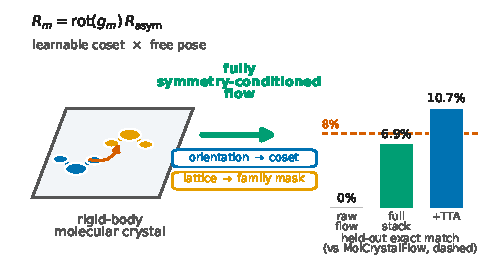
\includegraphics[width=\linewidth]{fig_toc.pdf}
%DIFDELCMD < %%%
\DIFdelend \DIFaddbegin 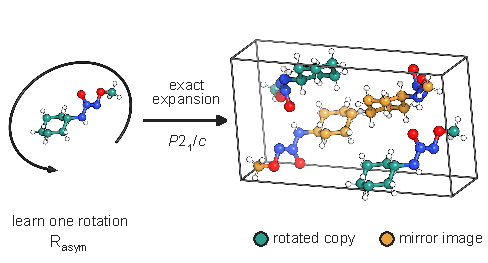
\includegraphics[width=3.25in]{fig_n3_toc}
\DIFaddend \end{tocentry}

\begin{abstract}
\noindent
Rigid-body \DIFdelbegin \DIFdel{flow matching reduces molecular-crystal structure prediction to a
lattice, fractional centroids, and per-molecule orientations on $\mathrm{SO}(3)$,
but current rigid-body molecular-crystal generators leave crystallographic
symmetry unconditioned, and symmetry-conditioned generation has been demonstrated
only for inorganic atomic sites. We show that the
per-molecule orientation target
factorizes as $R_m=\mathrm{rot}(g_m)\,R_{\text{asym}}$ into a
space-group-determined relative rotation, which a flow learns, and a
gauge-free
asymmetric-unit pose, which it cannot regress from packing. We turn this into a
deployable method: }\DIFdelend \DIFaddbegin \DIFadd{generative models of molecular crystals predict an orientation for every
molecule in the unit cell, although space-group symmetry fixes all of them once the
orientation of the asymmetric unit is known. We tested, in a preregistered benchmark, }\DIFaddend a
\DIFdelbegin \DIFdel{leak-free coset label---the generating }\DIFdelend \DIFaddbegin \DIFadd{flow model that predicts only the asymmetric-unit orientation and builds the crystal by
exact }\DIFaddend space-group \DIFdelbegin \DIFdel{operation, recoverable from a symmetry template at sampling time---conditions the orientation flow. On }\DIFdelend \DIFaddbegin \DIFadd{expansion. The task is orientation completion rather than crystal
structure prediction: for crystals with one molecule in the asymmetric unit, the true
lattice, space-group operations, asymmetric-unit centroid and rigid conformer are given,
and only the asymmetric-unit orientation is predicted. On \nN{} held-out crystals from the
}\DIFaddend Cambridge Structural Database\DIFdelbegin \DIFdel{crystals, deployable coset
conditioning lifts the held-out non-reference orientation loss by $41.1\%$ (versus
$27.5\%$ for a paired control), two-thirds of the way to a leaky-codebook oracle
($\sim\!48\%$); an $\mathrm{SO}(3)$-averaged objective closes the gap ($47.7\%$). Supplying the coset at generation collapses the end-to-end orientation error
sevenfold ($93.5^\circ\!\to\!13.4^\circ$), and the advantage widens with data.
Extending symmetry conditioning to the lattice---a crystal-family mask on an
$\mathrm{O}(3)$-invariant log-metric parametrization---gives,
to our knowledge, }\DIFdelend \DIFaddbegin \DIFadd{, scored once under a frozen protocol, }\DIFaddend the \DIFdelbegin \DIFdel{first fully symmetry-conditioned molecular-crystal flow. Paired with an
unsupervised symmetry-preserving packing finisher, a fully-ablated stack of levers
lifts held-out exact match from $0\%$ to $6.9\%$ (strict best-of-$10$, StructureMatcher $\text{stol}\,1.0$), at statistical parity with the symmetry-free
MolCrystalFlow ($\sim\!8\%$), reaching $10.7\%$ with orientation test-time
augmentation.
We report the contribution of each lever.
}\DIFdelend \DIFaddbegin \DIFadd{model reproduced
the experimental structure for \nOursPick{}~$\pm$~\nOursSd\% of crystals (one selected
structure per crystal; mean $\pm$ s.d.\ over three trained models). Three hypotheses were
tested, with a Holm correction for multiple comparisons. The model outperformed
MolCrystalFlow retrained on the same data and given the true lattice and the true
centroids of every molecule (H1: \nHOneDelta{} percentage points, pp; 95\% CI \nHOneCI)
and our previous architecture retrained on this task (H3: \nHThreeDelta{} pp \nHThreeCI),
so both hypotheses were supported, although both comparators, as retrained here, scored no
better than random orientations with the same selection step. A search over the
asymmetric-unit orientation with a universal interatomic potential, given the same
information, reproduced \nSearchPick\% of the structures, so the hypothesis comparing the
model with it (H2: \nHTwoDelta{} pp \nHTwoCI) was not supported.
}\DIFaddend \end{abstract}

% =====================================================================
\section{Introduction}
% =====================================================================
Crystal structure prediction (CSP) seeks the stable periodic packing of a chemical
system, and generative models have become a fast alternative to large ensembles of
\DIFdelbegin \DIFdel{density-functional relaxations}\DIFdelend \DIFaddbegin \DIFadd{energy evaluations}\DIFaddend , progressing from crystal diffusion autoencoders\cite{xie2022cdvae}
to joint equivariant diffusion\cite{jiao2023diffcsp} and \DIFdelbegin \DIFdel{Riemannian flow
matching\mbox{%DIFAUXCMD
\cite{miller2024flowmm,lipman2023flowmatching,chen2024riemannian}}\hskip0pt%DIFAUXCMD
, which
traverses a straight conditional path solvable in tens of steps}\DIFdelend \DIFaddbegin \DIFadd{flow
matching\mbox{%DIFAUXCMD
\cite{lipman2023flowmatching} }\hskip0pt%DIFAUXCMD
on Riemannian manifolds\mbox{%DIFAUXCMD
\cite{chen2024riemannian,miller2024flowmm}}\hskip0pt%DIFAUXCMD
}\DIFaddend . Rigid-body
factorization \DIFdelbegin \DIFdel{is especially attractive for }\DIFdelend \DIFaddbegin \DIFadd{suits }\DIFaddend molecular crystals: freezing each molecule's conformer \DIFdelbegin \DIFdel{collapses }\DIFdelend \DIFaddbegin \DIFadd{reduces
}\DIFaddend dozens of atomic coordinates to a \DIFdelbegin \DIFdel{single pose---a
lattice$L$}\DIFdelend \DIFaddbegin \DIFadd{lattice}\DIFaddend , a fractional centroid \DIFdelbegin \DIFdel{$c_m\in\mathbb{T}^3$, }\DIFdelend and an orientation \DIFdelbegin \DIFdel{$R_m\in\mathrm{SO}(3)$ per molecule---and supports the short sampling trajectories
characteristic of flow matching}\DIFdelend \DIFaddbegin \DIFadd{in
$\mathrm{SO}(3)$ for every molecule}\DIFaddend .

\DIFdelbegin \paragraph{\DIFdel{The gap.}} %DIFAUXCMD
\addtocounter{paragraph}{-1}%DIFAUXCMD
\DIFdel{This factorization introduces a per-molecule orientation variable on $\mathrm{SO}(3)$, and here the current generation of models underuses the available symmetry. MolCrystalFlow\mbox{%DIFAUXCMD
\cite{zeng2026molcrystalflow}}\hskip0pt%DIFAUXCMD
, a 2026 }\DIFdelend \DIFaddbegin \DIFadd{Space-group symmetry makes most of those orientations redundant, because in a crystal with
one molecule in the asymmetric unit ($Z'=1$) on a general position, the $K$ molecules of
the cell are the images of a single molecule under the $K$ operations $(W_k, t_k)$ of the
space group. Each copy's centroid and atoms follow from the asymmetric-unit molecule by the
operation, and an improper operation ($\det W_k=-1$) also mirrors the conformer, so the
orientation of the asymmetric unit, $R_{\text{asym}}$, fixes all $K$. Many classical
crystal structure prediction methods already work this way, placing the asymmetric unit in
a trial space group and generating the cell by symmetry\mbox{%DIFAUXCMD
\cite{price2023blindtest7}}\hskip0pt%DIFAUXCMD
, but
current learned }\DIFaddend rigid-body \DIFdelbegin \DIFdel{molecular-crystal flow with the identical
$\text{lattice}\times\mathbb{T}^3\times\mathrm{SO}(3)$ factorization, jointly
learns pose but
}\DIFdelend \DIFaddbegin \DIFadd{generators do not.
MolCrystalFlow\mbox{%DIFAUXCMD
\cite{zeng2026molcrystalflow} }\hskip0pt%DIFAUXCMD
generates an orientation for every molecule
and }\DIFaddend imposes no space-group constraint, and MOFFlow\cite{kim2025mofflow} \DIFdelbegin \DIFdel{flows rigid $\mathrm{SE}(3)$ poses
relying on
framework connectivity rather than a symmetry prior. Symmetry- }\DIFdelend \DIFaddbegin \DIFadd{generates the poses
of rigid building blocks of metal--organic frameworks. Space-group symmetry has been built into
generators of inorganic crystals, through Wyckoff positions or space-group-constrained
coordinates\mbox{%DIFAUXCMD
\cite{jiao2024diffcsppp,wyckoffdiff2025,symmcd2025,puny2025sgfm,mu2026nextcrystal}}\hskip0pt%DIFAUXCMD
;
none of these generates rigid molecules. For molecular crystals, SALA\mbox{%DIFAUXCMD
\cite{cai2026sala}
}\hskip0pt%DIFAUXCMD
generates conformation, lattice and packing end to end from a molecular graph and a space
group by evolving asymmetric-unit atomic coordinates. The present benchmark addresses a
narrower task: completing the orientation of a rigid asymmetric unit when the lattice,
operations and position are given.
}

\DIFadd{We ask whether the redundancy matters for learned models. Our model (OURS in the tables)
is a flow model that learns only $R_{\text{asym}}$ and expands it exactly. We compare it
with learned models that predict each copy independently and with classical searches, in
a benchmark whose hypotheses, statistics and claim rules were fixed in advance. Each arm
receives specified information about each crystal (Table~\ref{tab:info}), each learned
comparator is retrained on the same training set with its released code, }\DIFaddend and \DIFdelbegin \DIFdel{Wyckoff-conditioned generation, meanwhile, is proven only for }\emph{\DIFdel{inorganic
atomic sites}}%DIFAUXCMD
\DIFdel{: DiffCSP++\mbox{%DIFAUXCMD
\cite{jiao2024diffcsppp}}\hskip0pt%DIFAUXCMD
,
WyckoffDiff\mbox{%DIFAUXCMD
\cite{wyckoffdiff2025}}\hskip0pt%DIFAUXCMD
, SymmCD\mbox{%DIFAUXCMD
\cite{symmcd2025}}\hskip0pt%DIFAUXCMD
, and the 2026
NextCrystal\mbox{%DIFAUXCMD
\cite{mu2026nextcrystal} }\hskip0pt%DIFAUXCMD
all condition atom generation on a }\DIFdelend \DIFaddbegin \DIFadd{one scoring
script scores every arm once on \nN{} held-out crystals from the Cambridge Structural
Database (CSD)\mbox{%DIFAUXCMD
\cite{groom2016csd}}\hskip0pt%DIFAUXCMD
. The task is }\emph{\DIFadd{orientation completion}}\DIFadd{: given the
true lattice, the true }\DIFaddend space-group \DIFdelbegin \DIFdel{/Wyckoff template, but none conditions rigid-body molecular orientation. We close that gap and make the conditioning }\emph{\DIFdel{deployable}}%DIFAUXCMD
\DIFdel{. }%DIFDELCMD < 

%DIFDELCMD < %%%
\paragraph{\DIFdel{Contributions.}}
%DIFAUXCMD
\addtocounter{paragraph}{-1}%DIFAUXCMD
%DIFDELCMD < \begin{itemize}%%%
\DIFdel{\
}%DIFDELCMD < \item %%%
\DIFdel{A leak-free, template-available coset label (the generating operation
$h=g_mg_0^{-1}$, recovered from centroids alone) that conditions the orientation flow without seeing the target.
}%DIFDELCMD < \item %%%
\DIFdel{Deployable conditioning recovers two-thirds of }\DIFdelend \DIFaddbegin \DIFadd{operations, the true asymmetric-unit centroid and }\DIFaddend the
\DIFdelbegin \DIFdel{oracle-codebook
orientation benefit ($+41.1\%$ vs a $+27.5\%$ paired control); an
$\mathrm{SO}(3)$-averaged objective closes the rest ($+47.7\%$).
}%DIFDELCMD < \item %%%
\DIFdel{End-to-end,
supplying the coset collapses the orientation error $7\times$
($93.5^\circ\!\to\!13.4^\circ$), and the coset advantage }\emph{\DIFdel{widens}} %DIFAUXCMD
\DIFdel{with data.
}%DIFDELCMD < \item %%%
\DIFdel{A template-free path: a packing-only predictor whose top-$k$ covers the true
coset for $86\%$ of molecules at $k{=}5$, made usable by top-$k$ marginalization. }%DIFDELCMD < \item %%%
\DIFdel{Extending symmetry conditioning to the lattice (a crystal-family mask on a
log-metric parametrization) gives the first }\emph{\DIFdel{fully symmetry-conditioned}}
%DIFAUXCMD
\DIFdel{molecular-crystal flow ; composed with an unsupervised packing finisher and a
fully-ablated lever stack, it lifts exact match from $0\%$ to $6.9\%$ (strict
best-of-$10$}\DIFdelend \DIFaddbegin \DIFadd{rigid conformer of a $Z'=1$ crystal, predict $R_{\text{asym}}$. Because the lattice}\DIFaddend , \DIFdelbegin \DIFdel{$\text{stol}\,1.0$)---parity with MolCrystalFlow---and $10.7\%$ with orientation test-time augmentation.
}%DIFDELCMD < \end{itemize}
%DIFDELCMD < %%%
\DIFdelend \DIFaddbegin \DIFadd{space
group, $Z$, $Z'$ and molecular position are oracle inputs, this is not crystal structure
prediction.
}\DIFaddend 

%DIF <  =====================================================================
\DIFdelbegin \section{\DIFdel{Results and Discussion}}
%DIFAUXCMD
\addtocounter{section}{-1}%DIFAUXCMD
%DIF <  =====================================================================
\DIFdel{Throughout, SymMC-Flow denotes the rigid-body flow of the Methods section: a molecular crystal is carried as a lattice, a fractional centroid per molecule, and an orientation on $\mathrm{SO}(3)$, with a conditional flow-matching objective
trained jointly over the three manifolds. The }\emph{\DIFdel{coset label}} %DIFAUXCMD
\DIFdel{used below is }\DIFdelend \DIFaddbegin \DIFadd{Exact expansion with }\DIFaddend the \DIFdelbegin \DIFdel{generating space-group operation that maps a species' reference copy to copy $m$, assigned from fractional centroids against a symmetry template and never from the
observed rotation; its construction, the crystal-family latticemask, the finishing
stack, }\DIFdelend \DIFaddbegin \DIFadd{full operations, proper and improper, represents every test
crystal, whereas the parser of our previous work, which accepts proper rotations only,
cannot represent \nRLegacy{} of the \nN{} (Table~\ref{tab:repr}). Against learned models
the asymmetric-unit design is clearly ahead. MolCrystalFlow, retrained here, reproduces at
most \nMcfRGPick\% of the test structures and our previous architecture none, so both
preregistered comparisons with learned models (H1, H3) are supported. Both comparators
scored at the level of random orientations, however, which limits what these comparisons
show: OURS learned what the retrained models did not, }\DIFaddend and \DIFdelbegin \DIFdel{the corpus are specified in Methods}\DIFdelend \DIFaddbegin \DIFadd{the benchmark contains no working
learned comparator to measure a margin against. A physics-based search given the same
information is far more accurate (H2 not supported), since with the lattice and position
known only three rotational degrees of freedom remain and an accurate potential searched
over them finds nearly every structure. A learned asymmetric-unit model is therefore of
interest mainly as one component of a generator that must also produce the lattice and the
molecular position, a setting this benchmark does not test}\DIFaddend .

\DIFdelbegin \subsection{\DIFdel{The orientation decomposition}}%DIFAUXCMD
\addtocounter{subsection}{-1}%DIFAUXCMD
%DIFDELCMD < \label{sec:decomp}
%DIFDELCMD < %%%
\DIFdel{A molecule $m$ generated from the asymmetric unit by a }\DIFdelend %DIF >  =====================================================================
\DIFaddbegin \section{\DIFadd{Definitions and a Worked Example}}
%DIF >  =====================================================================
\DIFadd{Throughout, a crystal has one molecule in its asymmetric unit ($Z'=1$) on a general
position, so its unit cell holds $Z=K$ molecules, where $K$ is the number of operations of
the space group in the crystal's own setting. We use the following terms.
}\begin{description}\item[\DIFadd{Operation.}] \DIFadd{A }\DIFaddend space-group \DIFdelbegin \DIFdel{operation with rotation part $\mathrm{rot}(g_m)$ has absolute pose
}\begin{displaymath}
\DIFdel{R_m = \mathrm{rot}(g_m)\,R_{\text{asym}},
%DIFDELCMD < \label{eq:decomp}%%%
}\end{displaymath}%DIFAUXCMD
\DIFdel{where $R_{\text{asym}}$ }\DIFdelend \DIFaddbegin \DIFadd{operation $(W_k,t_k)$ maps fractional coordinates
$c\mapsto W_kc+t_k$. It is }\emph{\DIFadd{proper}} \DIFadd{if $\det W_k=+1$ (a rotation or screw rotation)
and }\emph{\DIFadd{improper}} \DIFadd{if $\det W_k=-1$ (an inversion, reflection, glide reflection or
rotoinversion).
}\item[\DIFadd{Asymmetric-unit molecule and copies.}] \DIFadd{The asymmetric-unit molecule is one molecule
of the cell, with fractional centroid $c_0$ and a rigid conformer (its atom positions
about the centroid, held at the experimental geometry). The $K$ molecules of the cell are
its }\emph{\DIFadd{copies}}\DIFadd{: copy $k$ }\DIFaddend is the \DIFdelbegin \DIFdel{orientation of the asymmetric unit in the cell. The
first factor is fixed by the space group and shared across crystals; the second is
a free, per-crystal choice. Because the body-frame gauge is arbitrary, }\DIFdelend \DIFaddbegin \DIFadd{image of the asymmetric-unit molecule under operation
$k$, and copy 1 (the identity) is the asymmetric-unit molecule itself.
}\item[\DIFadd{Orientation and $R_{\text{asym}}$.}] \DIFadd{An orientation is a rotation in $\mathrm{SO}(3)$
that places the conformer in the cell; }\DIFaddend $R_{\text{asym}}$ \DIFdelbegin \DIFdel{carries no consistent signal tied to composition or packing:
trained directly on $R_m$, an absolute-orientation head never leaves its
predict-zero floor ($\mathbb{E}\lVert u_R\rVert^2\!\approx\!5.24$) while the lattice and centroid heads converge normally. The empirical distribution is
consistent with this---absolute reference-copy orientations track the Haar-uniform
density on $\mathrm{SO}(3)$ (mean geodesic angle $122.6^\circ$ against the Haar
expectation $126.5^\circ$; Kolmogorov--Smirnov $D=0.04$) }\DIFdelend \DIFaddbegin \DIFadd{is the orientation of the
asymmetric-unit molecule.
}\item[\DIFadd{Handedness.}] \DIFadd{An improper operation turns the conformer into its mirror image. For a
chiral conformer this is the opposite enantiomer, so the copy has the opposite handedness to
the asymmetric-unit molecule.
}\item[\DIFadd{Exact expansion.}] \DIFadd{Building all $K$ copies from $c_0$}\DIFaddend , \DIFdelbegin \DIFdel{and a supervised probe
trained to predict }\DIFdelend $R_{\text{asym}}$ \DIFdelbegin \DIFdel{from lattice, centroid arrangement, conformer,
and space group does not beat the best feature-free constant (Supporting
Information). We therefore state the claim operationally and narrowly:
}\DIFdelend \DIFaddbegin \DIFadd{and the
conformer by applying each operation to the atoms (eq~\ref{eq:expand} in Methods). Because
the operation acts on atoms, an improper operation produces the mirrored copy directly; no
rotation is assigned to it.
}\item[\DIFadd{Orientation flow.}] \DIFadd{A generative model that turns random rotations into a predicted
rotation by integrating a learned velocity field on $\mathrm{SO}(3)$. OURS draws
}\DIFaddend $R_{\text{asym}}$ \DIFdelbegin \DIFdel{is not predictable from the
conditioning available here, not that
orientation is unlearnable in principle---a richer descriptor such as
hydrogen-bond topology or dipole alignment could in principle expose residual
signal}\DIFdelend \DIFaddbegin \DIFadd{this way (Methods)}\DIFaddend .
\DIFaddbegin \end{description}
\DIFaddend 

\DIFdelbegin \DIFdel{To isolate the learnable factor we re-gauge each crystal so the first copy of every
species is a reference ($R=I$) and the remaining copies carry only the relative
rotation $R'_m=R_mR_0^{-1}$, which cancels }\DIFdelend \DIFaddbegin \paragraph{\DIFadd{Worked example.}} \DIFadd{Figure~\ref{fig:worked} shows a training-set crystal in
$P2_1/c$ ($K=4$; CSD refcode LAJKOX, C$_7$H$_{15}$N$_3$O$_2$). Its four operations are the
identity, a twofold screw rotation (proper), an inversion (improper) and a glide reflection
(improper). Given }\DIFaddend $R_{\text{asym}}$\DIFdelbegin \DIFdel{and leaves the
reconstructed crystalunchanged. Splitting the orientation loss into reference
copies (target $I$)
and non-reference copies (the symmetry-determined targets) and
reporting the latter---which cannot be earned by predicting the identity---the
held-out non-reference loss drops by $27.5\pm2.7\%$ over three seeds
(Table~\ref{tab:twobytwo}), identically under noised and clean conditioning, so the
signal rides on the space group (conditioned directly)and the coarse centroid
arrangement.
A stricter species-grouped split that keeps every crystal sharing a
species on one side of the partition gives $28.5\pm2.9\%$, ruling out species
leakage between training and validation. The floor of the absolute target and the descent of the relative target together confirm Eq.~\eqref{eq:decomp}: the only
learnable content in $R_m$ is the part that survives cancellation of
$R_{\text{asym}}$.
This is a diagnostic; the coset construction given in Methods
turns it into a deployable method. }\DIFdelend \DIFaddbegin \DIFadd{, the identity copy is the asymmetric-unit molecule, the
screw copy is its rotated image, and the inversion and glide copies are its mirror images.
The given centroid and operations fix where each copy sits and which copies are mirrored,
and one predicted rotation (three numbers) then fixes all four orientations. A model that
predicts an orientation for every copy must learn these relations from data and needs a
separate mirrored conformer for each improper copy; a model that predicts only
$R_{\text{asym}}$ obtains them exactly from the operations.
}\DIFaddend 

\DIFdelbegin %DIFDELCMD < \begin{table}[t]\centering
%DIFDELCMD < \caption{Held-out non-reference orientation loss (untrained $\rightarrow$ trained)
%DIFDELCMD < across orientation target and conditioning. The absolute pose floors; the relative
%DIFDELCMD < (symmetry-determined) orientation is learnable and robust to conditioning noise.}
%DIFDELCMD < \label{tab:twobytwo}
%DIFDELCMD < \begin{tabular}{lcc}\toprule
%DIFDELCMD < target & noised conditioning & clean packing \\\midrule
%DIFDELCMD < absolute $R_m$  & $5.37\!\rightarrow\!5.18$ ($+3.3\%$) & $5.35\!\rightarrow\!5.18$ ($+3.3\%$) \\
%DIFDELCMD < relative $R'_m$ & $5.37\!\rightarrow\!3.91$ ($+27.1\%$) & $5.37\!\rightarrow\!3.94$ ($+26.7\%$) \\
%DIFDELCMD < \bottomrule
%DIFDELCMD < \end{tabular}
%DIFDELCMD < \end{table}
%DIFDELCMD < %%%
\DIFdelend \DIFaddbegin \begin{figure}
\centering
\IfFileExists{figures/fig_n3_worked_example.pdf}{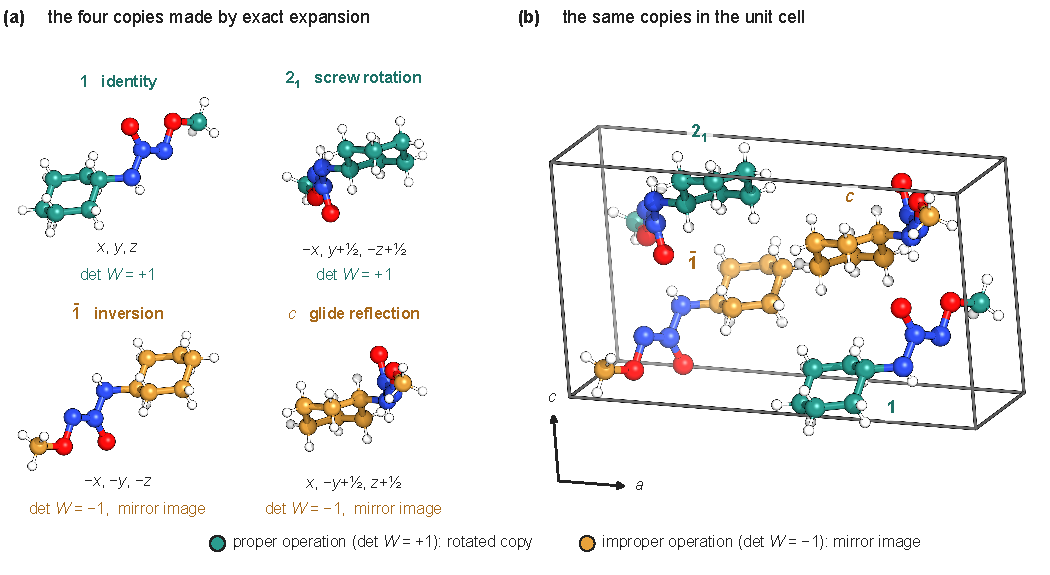
\includegraphics[width=\linewidth,height=0.72\textheight,keepaspectratio]{fig_n3_worked_example}}{\TODO{figure: worked example}}
\caption{Worked example: training crystal LAJKOX ($P2_1/c$, $K=4$). (a) The four copies that
exact expansion (eq~\ref{eq:expand}) builds from the asymmetric-unit molecule, which is the
identity copy. Copy $k$ has centroid $c_k=W_kc_0+t_k$ and atoms placed by
$C_kR_{\text{asym}}$ about it, so one rotation, $R_{\text{asym}}$, fixes every copy; each
operation is given in the crystal's CSD setting. Copies made by proper operations
($\det W_k=+1$; teal carbon atoms) are rotated images of the asymmetric-unit molecule, and
copies made by improper operations ($\det W_k=-1$; amber carbon atoms) are its mirror images,
because $C_k$ then includes a reflection. (b) The same copies in the unit cell, each tagged
with its operation, seen obliquely from near the $b$ axis; every tile in (a) is drawn from
this viewpoint. The cell is outlined with its origin shifted by $-c/4$ so that every copy's
centroid lies inside it. N, O and H atoms are shown in standard colors.}
\label{fig:worked}
\end{figure}
\DIFaddend 

\DIFdelbegin \subsection{\DIFdel{Deployable coset conditioning recovers the oracle benefit}}
%DIFAUXCMD
\addtocounter{subsection}{-1}%DIFAUXCMD
%DIFDELCMD < \label{sec:gate}
%DIFDELCMD < %%%
\DIFdel{Table~\ref{tab:gate} gives the main result. A paired no-coset control reproduces
$+27.5\%$; the deployable coset reaches $+41.1\%$---two-thirds }\DIFdelend \DIFaddbegin \paragraph{\DIFadd{Terms from the earlier version of this work.}} \DIFadd{Each molecule's conformer is
stored in its own coordinate frame (the }\emph{\DIFadd{body frame}}\DIFadd{), and the choice of which
orientation counts as the identity (the }\emph{\DIFadd{gauge}}\DIFadd{) is arbitrary. Our earlier manuscript
chose one copy as the }\emph{\DIFadd{reference copy}} \DIFadd{and }\emph{\DIFadd{re-gauged}} \DIFadd{the crystal, expressing
each copy's orientation $R_k$ relative to the reference as $R_kR_0^{\top}$. It also
conditioned the model on a }\emph{\DIFadd{coset label}}\DIFadd{, which identified the operation that generates
each copy (the $K$ operations represent the cosets }\DIFaddend of the \DIFdelbegin \DIFdel{way to
the $\sim\!48\%$ leaky ceiling---and the
$\mathrm{SO}(3)$-averaged objective ($K{=}4$)reaches $+47.7\%$, statistically level with the ceiling.
The benefit that a
target-derived codebook could only }\emph{\DIFdel{upper-bound}} %DIFAUXCMD
\DIFdel{is realized here by a label a
sampler actually has. }%DIFDELCMD < 

%DIFDELCMD < \begin{table}[t]\centering
%DIFDELCMD < \caption{Held-out non-reference orientation-loss drop, mean$\pm$s.d.\ (3 seeds).
%DIFDELCMD < The deployable coset is leak-free and available from a template; the leaky codebook
%DIFDELCMD < (index clustered from the target) is an upper bound.}
%DIFDELCMD < \label{tab:gate}
%DIFDELCMD < \begin{tabular}{lcc}\toprule
%DIFDELCMD < configuration & non-ref.\ loss drop & deployable? \\\midrule
%DIFDELCMD < no-coset control (baseline)            & $27.5\pm2.7\%$ & --- \\
%DIFDELCMD < deployable coset ($K{=}1$)             & $41.1\pm3.4\%$ & yes \\
%DIFDELCMD < \quad + $\mathrm{SO}(3)$-averaged      & $47.7\pm3.9\%$ & yes \\
%DIFDELCMD < leaky codebook (oracle upper bound)    & $\sim48\%$      & no  \\\bottomrule
%DIFDELCMD < \end{tabular}
%DIFDELCMD < \end{table}
%DIFDELCMD < 

%DIFDELCMD < %%%
\subsection{\DIFdel{The coset makes orientation work end-to-end}}%DIFAUXCMD
\addtocounter{subsection}{-1}%DIFAUXCMD
%DIFDELCMD < \label{sec:e2e}
%DIFDELCMD < %%%
\DIFdel{Sampling all three manifolds from the prior (full de-novo generation), supplying
the
coset at generation collapses the median orientation error from $93.5^\circ$
(the same model with the coset withheld)to $13.4^\circ$---a $7\times$
reduction---while the centroid error is unchanged ($0.346$ vs $0.345$; the coset
does not touch it) and neither reaches exact match ($0\%$; lattice $0.44$ /
centroid $0.35$ dominate). The coset thus makes the orientation component work
end-to-end; joint lattice--centroid generation is the remaining exact-match
bottleneck.
}%DIFDELCMD < 

%DIFDELCMD < %%%
\subsection{\DIFdel{Orientation-isolated reconstruction}}%DIFAUXCMD
\addtocounter{subsection}{-1}%DIFAUXCMD
%DIFDELCMD < \label{sec:orientiso}
%DIFDELCMD < %%%
\DIFdel{A drop in flow-matching loss need not correspond to correct geometry. Holding the
true lattice, centroid, and conformer fixed and sampling only the }\DIFdelend \DIFaddbegin \DIFadd{lattice translations in the space
group). For a proper operation $R_kR_0^{\top}=C_k$ (eq~\ref{eq:expand}), so the relative
orientation is fixed analytically by the operation; for an improper operation the relative
orientation is not a rotation of the same conformer at all. The earlier manuscript
interpreted the reduced loss on these symmetry-determined relative targets as evidence that
orientation is learnable; we withdraw that interpretation. In its }\DIFaddend coset-conditioned
\DIFdelbegin \DIFdel{$\mathrm{SO}(3)$ field,
the flow reconstructs $27.5\%$ of held-out multi-copy
packings (best-of-$8$) , rising to $37.4\%$ at looser but oracle-validated
tolerances, with a median non-reference orientation error of $41.1^\circ$; the
oracle (true orientation) matches every structure (Table~\ref{tab:tolsweep}). The
symmetry-relative rotations cluster near $180^\circ$ (the dominant $P2_1/c$,
$P\bar1$ operations)\mbox{%DIFAUXCMD
\cite{groom2016csd}}\hskip0pt%DIFAUXCMD
, so a single deterministic integration
collapses to the conditional mean and best-of-$k$ is the correct read of a
multimodal target}\DIFdelend \DIFaddbegin \DIFadd{experiments, the label supplied the generating operation explicitly. The present design learns only $R_{\text{asym}}$ and lets the
operations supply everything else exactly. The comparison arm iv-P (H3) is our previous
architecture retrained on this task: it receives per-copy operation labels and mirrored
conformers and predicts every copy's absolute orientation. The earlier manuscript's
relative-target experiment was not rerun}\DIFaddend .

\DIFdelbegin %DIFDELCMD < \begin{table}[t]\centering
%DIFDELCMD < \caption{Orientation-isolated reconstruction (coset-conditioned, best-of-$8$; true
%DIFDELCMD < lattice, centroid, and conformer supplied, only $\mathrm{SO}(3)$ sampled):
%DIFDELCMD < \textsc{StructureMatcher} match rate across the (length, site) tolerance grid on
%DIFDELCMD < the held-out set. The oracle (true orientation) matches throughout.}
%DIFDELCMD < \label{tab:tolsweep}
%DIFDELCMD < \begin{tabular}{lccc}\toprule
%DIFDELCMD < (ltol, stol) & $(0.2,0.2)$ & $(0.3,0.5)$ & $(0.5,0.7)$ \\\midrule
%DIFDELCMD < coset-conditioned & $4.6\%$  & $27.5\%$ & $37.4\%$ \\
%DIFDELCMD < oracle (true $R$) & $100\%$  & $100\%$  & $100\%$  \\\bottomrule
%DIFDELCMD < \end{tabular}
%DIFDELCMD < \end{table}
%DIFDELCMD < %%%
\DIFdelend %DIF >  =====================================================================
\DIFaddbegin \section{\DIFadd{Results and Discussion}}
%DIF >  =====================================================================
\subsection{\DIFadd{Benchmark design}}
\begin{table}[t]
\caption{Information given to each arm. For the MolCrystalFlow (MCF) arms,
``copies'' means $z_{\mathrm{MCF}}$, the number of molecules in the exported MCF
cell: $K$ for primitive lattices and $K/\mathrm{mult}$ for centered ones, where
mult is the centering multiplicity (lattice points per cell). MCF-R is not given the operations, but
spglib on the true centroids, keeping the operations consistent with each copy's
handedness, recovers the copy-to-copy rotations uniquely in 198 of 200 DEV-TEST (development-set)
crystals (the truth is among the candidates in the other 2). H1 therefore tests
explicit, enforced symmetry together with our learner; the ii-S ablation
separates the two.}
\label{tab:info}
\small
\begin{tabular}{@{}p{2.3cm}p{2.9cm}p{2.6cm}p{3.0cm}p{2.5cm}@{}}
\toprule
 & OURS and CLASSICAL & iv-P (previous architecture) & MCF-R and MCF-R+G & MCF-A (context) \\
\midrule
lattice & true & true & true (primitive if centered) & generated \\
centroids & $c_0$ true; copies from the operations & all $K$ true & all $z_{\mathrm{MCF}}$ true & generated \\
space-group operations & given, enforced exactly & given as per-copy operation labels & not given (recoverable; see caption) & not given \\
copy count & $K$, via the operations & $K$ given & $z_{\mathrm{MCF}}$ given & $z_{\mathrm{MCF}}$ given \\
per-copy handedness & $\det W_k$ & mirrored per-copy conformer & mirrored per-copy conformer and flag $\chi$ & as MCF-R \\
predicted & $R_{\mathrm{asym}}$ (3 degrees of freedom) & $K$ orientations & $z_{\mathrm{MCF}}$ orientations & lattice, centroids, orientations \\
copies built by & exact expansion & independent outputs, coupled by attention & independent outputs & independent outputs \\
\bottomrule
\end{tabular}
\end{table}
%DIF >  src: tasks/n3_protocol.md:43-64
\DIFaddend 

\DIFdelbegin \subsection{\DIFdel{Template-free deployment via top-$k$ marginalization}}%DIFAUXCMD
\addtocounter{subsection}{-1}%DIFAUXCMD
%DIFDELCMD < \label{sec:free}
%DIFDELCMD < %%%
\DIFdel{The packing-only predictor is
$39.5\%$ top-1 ($4\times$ the $10.3\%$ majority), but
the true coset is in its top-3 for $75.8\%$ of molecules, top-5 for $85.6\%$}\DIFdelend \DIFaddbegin \DIFadd{Table~\ref{tab:info} lists what each arm is given and what it predicts, and the Methods
describe each arm in full. OURS is a flow model over $R_{\text{asym}}$ that draws $16$ candidate
orientations per crystal, expands each one exactly with the given operations, and keeps
the candidate with the lowest steric Lennard-Jones (LJ) energy. The comparators are
MolCrystalFlow retrained on our training set and given the true lattice and the true
centroids of all copies (MCF-R), the same with a deployable symmetry scan of its output
(MCF-R+G)}\DIFaddend , \DIFdelbegin \DIFdel{top-10 for $90.9\%$ (Table~\ref{tab:cover}) . The signal is present; the argmax
merely cannot commit. Marginalizing the top-5 pulls the predicted-coset orientation error from $64.8^\circ$ (top-1) to $51.2^\circ$, toward the $41.1^\circ$ template
ceiling. At the larger corpus (\S\ref{sec:scale}) the predictor sharpens only to
$43.1\%$ top-1 and its predicted cosets still reconstruct below template grade, so
closing this residual---a sharper predictor or per-molecule combinatorial
search---remains the open problem.
}\DIFdelend \DIFaddbegin \DIFadd{three classical arms that are given exactly what OURS is given (random
orientations with the same LJ pick, iii-u; a short minimization of those orientations under
a steric potential, the ``steric press'', iii-p; and a search with a
universal interatomic potential, iii-s), and our previous architecture (iv-P), which
predicts all $K$ orientations from per-copy operation labels.
}\DIFaddend 

\DIFdelbegin %DIFDELCMD < \begin{table}[t]\centering
%DIFDELCMD < \caption{Predictor top-$k$ coverage: true coset in the top $k$ predictions
%DIFDELCMD < (non-reference molecules, $n{=}438$).}
%DIFDELCMD < \label{tab:cover}
%DIFDELCMD < \begin{tabular}{lcccc}\toprule
%DIFDELCMD < top-$k$ & 1 & 3 & 5 & 10 \\\midrule
%DIFDELCMD < coverage & $39.5\%$ & $75.8\%$ & $85.6\%$ & $90.9\%$ \\\bottomrule
%DIFDELCMD < \end{tabular}
%DIFDELCMD < \end{table}
%DIFDELCMD < 

%DIFDELCMD < %%%
\subsection{\DIFdel{Scale}}%DIFAUXCMD
\addtocounter{subsection}{-1}%DIFAUXCMD
%DIFDELCMD < \label{sec:scale}
%DIFDELCMD < %%%
\DIFdel{Retraining the full pipeline on a $2{,}539$-crystal CSD corpus ($2{,}464$
multi-copy after re-gauge; $2{,}168$ train / $296$ validation; $320$ distinct
operation-cosets), roughly $2.2\times$ the diagnostic set, sharpens every
orientation metric while leaving the packing bottleneck untouched
(Table~\ref{tab:scale}). The deployable-coset gate does not merely hold: the non-reference loss drop rises to $54.3\pm0.8\%$ against a paired no-coset control at
$36.8\pm2.1\%$}\DIFdelend \DIFaddbegin \DIFadd{The headline metric is picked@1: the fraction of crystals whose one selected structure
matches the unrelaxed experimental structure under pymatgen's
}\texttt{\DIFadd{StructureMatcher}}\DIFadd{\mbox{%DIFAUXCMD
\cite{ong2013pymatgen} }\hskip0pt%DIFAUXCMD
with default tolerances. The matcher does
not distinguish enantiomorphs, so a match does not certify the absolute configuration;
under exact expansion, each copy's handedness comes from the supplied operations. The
metric is averaged over three independently trained models (seeds). Differences are paired over crystals,
in percentage points (pp), with bias-corrected and accelerated (BCa) bootstrap 95\%
confidence intervals. A two-stage interval that also resamples seeds is reported beside
each, and the three hypotheses are corrected for multiple comparisons with Holm's
procedure. The confirmatory set}\DIFaddend , \DIFdelbegin \emph{\DIFdel{widening}} %DIFAUXCMD
\DIFdel{the coset advantage from $+13.6$ to $+17.5$
percentage points---the benefit is a property of the factorization, not a
small-data artifact. End-to-end with the coset supplied, the median orientation error falls to $4.3^\circ$ (from $13.4^\circ$), and orientation-isolated
reconstruction climbs to $56.8\%$ best-of-$8$ at $31.7^\circ$ (from $27.5\%$ at
$41.1^\circ$). Exact end-to-end match remains $0\%$ with the
lattice ($0.42$) and
centroid ($0.35$) component errors essentially unchanged: scaling data sharpens
orientationbut does not move the joint lattice--centroid bottleneck.
}\DIFdelend \DIFaddbegin \DIFadd{TEST-B,
holds \nN{} crystals. A second set, DEV-TEST, was used during development and is reported
in the Supporting Information as non-confirmatory.
}\DIFaddend 

\DIFdelbegin %DIFDELCMD < \begin{table*}[t]\centering
%DIFDELCMD < \caption{Diagnostic ($N\!\approx\!1.1$k) vs.\ scale ($N\!=\!2.5$k) corpus:
%DIFDELCMD < orientation metrics sharpen with data while end-to-end exact match stays
%DIFDELCMD < lattice/centroid-limited. The gate is the held-out non-reference orientation-loss
%DIFDELCMD < drop (deployable coset, $K{=}1$); orientation-isolated match is best-of-$8$ with
%DIFDELCMD < true lattice$+$centroid supplied.}
%DIFDELCMD < \label{tab:scale}
%DIFDELCMD < \begin{tabular}{lcc}\toprule
%DIFDELCMD < metric & diagnostic & scale \\\midrule
%DIFDELCMD < coset gate: non-ref.\ loss drop (deployable) & $41.1\%$ & $\mathbf{54.3\%}$ \\
%DIFDELCMD < \quad paired no-coset control                & $27.5\%$ & $36.8\%$ \\
%DIFDELCMD < \quad coset advantage                        & $+13.6$ pp & $\mathbf{+17.5}$ pp \\
%DIFDELCMD < end-to-end orientation error (coset supplied)& $13.4^\circ$ & $\mathbf{4.3^\circ}$ \\
%DIFDELCMD < orient-isolated match (best-of-$8$)          & $27.5\%$ & $\mathbf{56.8\%}$ \\
%DIFDELCMD < orient-isolated orientation error            & $41.1^\circ$ & $\mathbf{31.7^\circ}$ \\
%DIFDELCMD < predictor top-1 (majority baseline)          & $39.5\%$ ($10.3\%$) & $43.1\%$ ($10.4\%$) \\
%DIFDELCMD < end-to-end exact match                       & $0\%$ & $0\%$ \\\bottomrule
%DIFDELCMD < \end{tabular}
%DIFDELCMD < \end{table*}
%DIFDELCMD < 

%DIFDELCMD < %%%
\subsection{\DIFdel{Comparison to rigid-body baselines}}%DIFAUXCMD
\addtocounter{subsection}{-1}%DIFAUXCMD
%DIFDELCMD < \label{sec:bench}
%DIFDELCMD < %%%
\DIFdel{To make the contribution legible to the same reviewers, }\DIFdelend \DIFaddbegin \subsection{\DIFadd{Representability}}
\DIFadd{Before any sampling, }\DIFaddend we \DIFdelbegin \DIFdel{re-score held-out
generations from the deployable coset model ($N\!\approx\!1.1$k) in MolCrystalFlow's exact units\mbox{%DIFAUXCMD
\cite{zeng2026molcrystalflow}}\hskip0pt%DIFAUXCMD
: pymatgen
}\textsc{\DIFdel{StructureMatcher}} %DIFAUXCMD
\DIFdelend \DIFaddbegin \DIFadd{counted the test crystals whose }\emph{\DIFadd{true}} \DIFadd{structure each
representation can emit }\DIFaddend (\DIFdelbegin \DIFdel{$\text{ltol}{=}0.3$, $\text{atol}{=}10^\circ$, site
tolerance swept $0.5$--$1.2$), best-of-$10$ match rate, and the relative
cell-volume deviation (RMAD) over all ten samples. We pair a de-novo pass (no
template, coset off---the MolCrystalFlow }\DIFdelend \DIFaddbegin \DIFadd{Table~\ref{tab:repr}). Exact expansion with the full operations
represents all of them by construction, as does MolCrystalFlow's per-copy representation,
which the MCF arms of this benchmark use. Our previous parser aligned every copy to one
conformer by proper rotations only (the ``legacy det+1 pipeline''). The legacy det+1
pipeline cannot represent \nRLegacy}\DIFaddend /\DIFdelbegin \DIFdel{MOFFlow regime) against our symmetry-conditioned pass (coset on)on }\emph{\DIFdel{identical}} %DIFAUXCMD
\DIFdel{prior draws
(Table~\ref{tab:bench}).
}%DIFDELCMD < 

%DIFDELCMD < %%%
\DIFdel{Two readings are deliberate and honest. First, end-to-end our diagnostic-scale
model is }\emph{\DIFdel{not}} %DIFAUXCMD
\DIFdel{competitive with the dedicated flows on either axis:
best-of-$10$ match is at floor ($0$--$0.8\%$) against MolCrystalFlow's $\sim\!6.8\%$
at $\text{stol}\,0.8$, and cell-volume RMAD ($\sim\!31\%$)lands between MOFFlow
($18.8\%$) and raw Genarris-3 ($59\%$)but well above MolCrystalFlow ($3.9\%$).
This is the lattice}\DIFdelend \DIFaddbegin \DIFadd{\nN{} test crystals (\nRLegacyCentro{} of the
centrosymmetric ones). The released MolCrystalFlow CSP driver cannot produce
\nRMixedMiss}\DIFaddend /\DIFdelbegin \DIFdel{centroid bottleneck of Table~\ref{tab:scale} now measured in
the baselines'units: our lattice and centroid heads are diagnostic-grade
}\emph{\DIFdel{before finishing}}%DIFAUXCMD
\DIFdel{, and \S\ref{sec:ladder} closes exactly this end-to-end
gap---to parity with MolCrystalFlow---with full lattice symmetry conditioning and
the finisher. Second, and the point of the paper, is the axis those baselines leave
}\emph{\DIFdel{unconditioned}}%DIFAUXCMD
\DIFdel{. The
coset barely moves RMAD ($32.9\%\!\to\!30.7\%$)---it
conditions orientation,
not packing---but on the same prior draws it collapses the
median best-of-$10$ orientation error from $103^\circ$ (de-novo)to $14^\circ$
(conditioned) . MolCrystalFlow and MOFFlow are both symmetry-free and have no such
lever; MolCrystalFlow is itself only }\emph{\DIFdel{competitive}} %DIFAUXCMD
\DIFdel{with the
space-group-conditioned Genarris-3, corroborating that symmetry conditioning---not
packing---is the remaining lever. Our contribution supplies exactly that for rigid-body orientation and composes with the strong packing these methods already
have. }\emph{\DIFdel{Caveat:}} %DIFAUXCMD
\DIFdel{identical matcher and match@$10$ as MolCrystalFlow, but our
corpus is a smaller CSD-derived molecular set(not Th\"urlemann}\DIFdelend \DIFaddbegin \DIFadd{\nRMixed{} mixed-handedness cells under the default StructureMatcher; a
homochiral approximant nevertheless matches \nRMixedApprox}\DIFaddend /\DIFdelbegin \DIFdel{OMC25) at diagnostic
scale---a comparable-task alignment, not a strict head-to-head.
}\DIFdelend \DIFaddbegin \DIFadd{\nRMixed{} at stol 0.5. A cell
counts as not producible when the lowest-RMSD homochiral approximant found by a 17-start
search (the 16 frozen starts plus the best automorphism rotation) does not match under the
primary matcher, a search result that does not prove that no homochiral cell could match.
Of the 351 crystals the legacy parser accepted, 342 match on oracle reconstruction
(Supporting Information). The MolCrystalFlow paper describes a mixed-handedness CSP
scenario whose code had not been released at the commit we used (3c493f8).
MolCrystalFlow's per-copy representation also covers $Z'>1$ and special-position crystals,
which our design excludes.
}\DIFaddend 

\DIFdelbegin %DIFDELCMD < \begin{table*}[t]\centering
%DIFDELCMD < \caption{Held-out generations in MolCrystalFlow's units (best-of-$10$;
%DIFDELCMD < \textsc{StructureMatcher} ltol$=0.3$/atol$=10^\circ$; RMAD$_{\mathrm{vol}}$ =
%DIFDELCMD < relative cell-volume deviation over all $10$ samples). Baseline rows are as
%DIFDELCMD < reported\cite{zeng2026molcrystalflow,kim2025mofflow} (Genarris-3 via the comparison
%DIFDELCMD < in ref~\citenum{zeng2026molcrystalflow}). Our end-to-end match and RMAD are
%DIFDELCMD < lattice/centroid-limited; the coset acts on orientation (last column)---the axis
%DIFDELCMD < the symmetry-free baselines omit.}
%DIFDELCMD < \label{tab:bench}
%DIFDELCMD < \begin{tabular}{lcccc}\toprule
%DIFDELCMD <  & \multicolumn{2}{c}{match@10} & RMAD$_{\mathrm{vol}}$ & orient.\ err. \\
%DIFDELCMD < \cmidrule(lr){2-3}
%DIFDELCMD < method & stol $0.8$ & stol $1.0$ & (all 10) & (best-of-10) \\\midrule
%DIFDELCMD < MolCrystalFlow (sym-free)\cite{zeng2026molcrystalflow} & $\sim\!6.8\%$ & $\sim\!8\%$ & $3.9\%$ & -- \\
%DIFDELCMD < MOFFlow (sym-free)\cite{kim2025mofflow}                & $\sim\!3.4\%$ & --          & $18.8\%$ & -- \\
%DIFDELCMD < Genarris-3 (sym-cond.)                                 & \multicolumn{2}{c}{comp.\ w/ MCF} & $59\%$ & -- \\\midrule
%DIFDELCMD < ours, de-novo (coset off)                              & $0\%$ & $0\%$   & $32.9\%$ & $103^\circ$ \\
%DIFDELCMD < ours, conditioned (coset on)                           & $0\%$ & $0.8\%$ & $30.7\%$ & $\mathbf{14^\circ}$ \\\bottomrule
%DIFDELCMD < \end{tabular}
%DIFDELCMD < \end{table*}
%DIFDELCMD < %%%
\DIFdelend \DIFaddbegin \begin{table}
\caption{Representability on TEST-B: crystals whose true structure each representation
can emit, under the primary matcher unless stated. (a) exact expansion with the full
operations (OURS and the classical arms; by construction); (b) MolCrystalFlow's per-copy
representation; (c) the information of the released MolCrystalFlow CSP driver, one
conformer and one handedness for all copies, as the lowest-RMSD homochiral approximant
found by a 17-start search (primary matcher, and stol 0.5); (d) crystals accepted by the
legacy det+1 parser, which accepts proper rotations only (part-file keep flag).}
\label{tab:repr}
\centering
\small
\begin{tabular}{lrrrrrr}
\toprule
crystals & $n$ & (a) & (b) & (c) & (c), stol 0.5 & (d) \\
\midrule
\inputrows{generated/n3_tableR.tex}
\bottomrule
\end{tabular}
\end{table}
\DIFaddend 

\DIFdelbegin \subsection{\DIFdel{From 0\% to parity: the exact-match lever ladder}}%DIFAUXCMD
\addtocounter{subsection}{-1}%DIFAUXCMD
%DIFDELCMD < \label{sec:ladder}
%DIFDELCMD < %%%
\DIFdel{The bottleneck the bench isolates---exact match at floor while orientation is
solved---is the question this section answers. Extending symmetry conditioning to
the lattice (\S\ref{sec:family}) restores the crystal-family geometry (generated
cell angles within $2^\circ$ of $90^\circ$ rise from $16\%$ to $73.6\%$,
matching
the reference $74.0\%$, ablation-isolated to the mask), but on its own does
}\emph{\DIFdel{not}} %DIFAUXCMD
\DIFdel{move exact match: the fully symmetry-conditioned flow still matches
$0/131$ held-out crystals. Fixing crystal family perfectly is necessary, not
sufficient---the residual blocker is close-packing }\emph{\DIFdel{precision}}%DIFAUXCMD
\DIFdel{.
The finishing
stack of \S\ref{sec:finish} supplies it, and we ablate each
lever independently
(Table~\ref{tab:ladder}, Fig. ~\ref{fig:ladder}; best-of-$10$, }\textsc{\DIFdel{StructureMatcher}} %DIFAUXCMD
\DIFdel{$\text{stol}\,1.0$,
coset on, $n{=}131$). }%DIFDELCMD < 

%DIFDELCMD < %%%
\DIFdel{The rigid-press finisher alone unblocks match ($0\%\!\to\!1.5\%$; the
raw flow
matches nothing); repairing the centroid head doubles it to $3.1\%$; corpus scale
($2.3\times$) improves the averaged metrics (RMAD, coset error) but leaves exact
match flat at $3.1\%$, mirroring the
orientation-scale finding of
\S\ref{sec:scale}.
Self-conditioning is the first lever to move the }\emph{\DIFdel{tight}}
%DIFAUXCMD
\DIFdel{tolerance, and scoring at MolCrystalFlow's own match @$10$ protocol with finer
($100$-step)sampling reaches $6.1\%$; AlphaFold-style recycling reaches
$\mathbf{6.9\%}$---statistical parity with MolCrystalFlow 's $\sim\!8\%$ ($95\%$ CI
$3.66$--$12.54$,
overlapping $8$), from a flow that matched zero.
An orientation-TTA
finishing pass (best-of-$30$, $3\times$ the finishing candidates) reaches
$\mathbf{10.7\%}$, above MolCrystalFlow, though at a larger finishing budget than
strict match@$10$. The median atom-RMSD to the reference falls from $1.02$ (raw)to
$0.77$ (best), }\DIFdelend \DIFaddbegin \subsection{\DIFadd{Headline results}}
\DIFadd{Table~\ref{tab:main} gives every arm, and Table~\ref{tab:hyp} the three hypotheses. OURS
reproduces \nOursPick~$\pm$~\nOursSd\% of the test structures (seeds \nOursSeeds\%), against
a random-orientation floor of \nFloorPick\% (OURS minus floor \nFloorDelta{} pp, \nFloorCI).
Much of this comes from choosing among the draws. A randomly chosen OURS draw matches
\nOursDraw\% of crystals and the LJ-selected draw \nOursPick\%, }\DIFaddend and \DIFdelbegin \DIFdel{cell-volume RMAD from $33\%$ to $21\%$. Diminishing returns are
explicit: recycling and orientation-TTA both refine positioning, so stacking them
($8.4\%$) underperforms TTA alone; corpus scale and cell relaxation add nothing to
match. These diminishing returns mark the effective ceiling for the current architecture. }\DIFdelend \DIFaddbegin \DIFadd{at least one of the 16
draws matches for \nOursAny\%. The selector alone does not account for the result, because
the same LJ pick over 16 random orientations (iii-u) reaches only \nHaarPick\%.
Figure~\ref{fig:forest} summarizes every contrast.
}\DIFaddend 

\DIFdelbegin %DIFDELCMD < \begin{figure}[t]\centering
%DIFDELCMD < 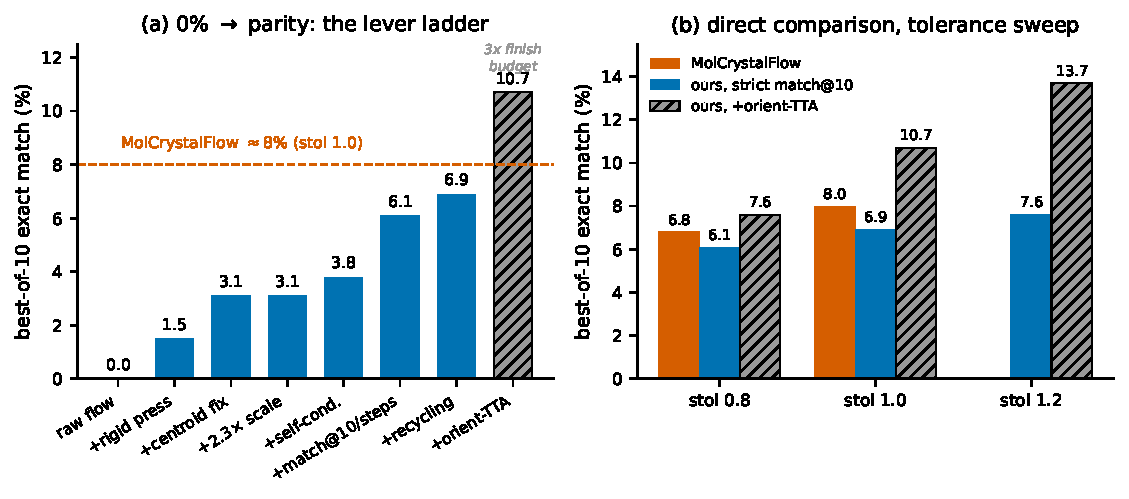
\includegraphics[width=\linewidth]{fig3_ladder.pdf}
%DIFDELCMD < \caption{The exact-match lever ladder (coset on, $n{=}131$, best-of-$10$,
%DIFDELCMD < \textsc{StructureMatcher}). \textbf{(a)}~Each lever added in turn lifts held-out
%DIFDELCMD < exact match from $0\%$ (raw fully symmetry-conditioned flow) to $6.9\%$ at
%DIFDELCMD < $\text{stol}\,1.0$, at parity with MolCrystalFlow (dashed); the orientation-TTA
%DIFDELCMD < pass reaches $10.7\%$ at a $3\times$ finishing budget. \textbf{(b)}~The best
%DIFDELCMD < configuration across the site-tolerance sweep against MolCrystalFlow's reported
%DIFDELCMD < match@$10$: strict match@$10$ is at parity, orientation-TTA clears it.}
%DIFDELCMD < \label{fig:ladder}
%DIFDELCMD < \end{figure}
%DIFDELCMD < %%%
\DIFdelend \DIFaddbegin \DIFadd{The orientation errors show where the model succeeds. The error is the angle between the
selected and the experimental asymmetric-unit orientation, minimized over the molecule's
proper point group. Averaged over the three seeds, the median error of OURS is
\nOursGeoMed$^\circ$, close to the \nHaarGeoMed$^\circ$ of random orientations with the same
LJ pick (iii-u), whereas its tenth percentile is \nOursGeoQten$^\circ$ against
\nHaarGeoQten$^\circ$. The model's advantage
therefore lies in a minority of crystals that it orients nearly correctly, while its typical
error is close to that of random orientations. For the \nOursAny\% of crystals with a
matching draw among the 16, a better selector could still raise the rate; for the others,
the proposals themselves would have to improve.
}\DIFaddend 

\DIFdelbegin %DIFDELCMD < \begin{table*}[t]\centering
%DIFDELCMD < \caption{Exact-match lever ladder: held-out best-of-$10$ match (coset on, $n{=}131$;
%DIFDELCMD < \textsc{StructureMatcher} ltol$=0.3$/atol$=10^\circ$; frozen cell). Each row adds
%DIFDELCMD < one lever to the row above. Strict match@$10$ is $10$ model draws $\times$ single
%DIFDELCMD < finish; orientation-TTA is best-of-$30$ ($3\times$ finishing candidates).
%DIFDELCMD < MolCrystalFlow is the symmetry-free rigid-body flow.}
%DIFDELCMD < \label{tab:ladder}
%DIFDELCMD < \begin{tabular}{lccl}\toprule
%DIFDELCMD < lever & stol $0.8$ & stol $1.0$ & note \\\midrule
%DIFDELCMD < raw flow (fully sym-conditioned)        & $0.0\%$ & $0.0\%$ & family mask + coset, no polish \\
%DIFDELCMD < \quad + rigid-press finisher            & $1.5\%$ & $1.5\%$ & unsupervised physical packing \\
%DIFDELCMD < \quad + centroid fix (OT + prior)       & $1.5\%$ & $3.1\%$ & repairs centroid head \\
%DIFDELCMD < \quad + $2.3\times$ scale               & $1.5\%$ & $3.1\%$ & moves RMAD/coset, not match \\
%DIFDELCMD < \quad + self-conditioning               & $3.05\%$& $3.8\%$ & first to move tight tolerance \\
%DIFDELCMD < \quad + match@$10$ + steps$=100$        & $4.6\%$ & $6.1\%$ & MCF protocol + finer sampling \\
%DIFDELCMD < \quad + recycling                       & $\mathbf{6.1\%}$ & $\mathbf{6.9\%}$ & best strict; parity w/ MCF \\
%DIFDELCMD < \quad + orientation-TTA (best-of-$30$)  & $7.6\%$ & $\mathbf{10.7\%}$ & $3\times$ finish budget \\\midrule
%DIFDELCMD < MolCrystalFlow (sym-free)\cite{zeng2026molcrystalflow} & $\sim\!6.8\%$ & $\sim\!8\%$ & reference \\
%DIFDELCMD < \bottomrule
%DIFDELCMD < \end{tabular}
%DIFDELCMD < \end{table*}
%DIFDELCMD < %%%
\DIFdelend \DIFaddbegin \begin{figure}
\centering
\IfFileExists{figures/fig_n3_forest.pdf}{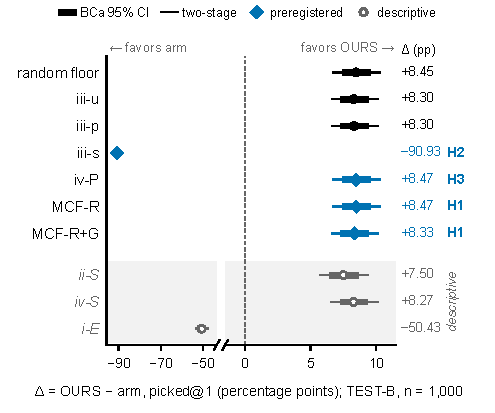
\includegraphics[width=\linewidth]{fig_n3_forest}}{\TODO{figure: forest plot}}
\caption{OURS minus each arm on TEST-B ($n=1{,}000$; percentage points): paired BCa 95\% CI
(thick) and two-stage seed interval (thin); the axis is broken. H1--H3 mark the
preregistered contrasts; ii-S, iv-S and i-E are descriptive.}
\label{fig:forest}
\end{figure}
\DIFaddend 

\DIFdelbegin \subsection{\DIFdel{Limitations}}%DIFAUXCMD
\addtocounter{subsection}{-1}%DIFAUXCMD
%DIFDELCMD < \label{sec:limits}
%DIFDELCMD < %%%
\DIFdel{Evaluation is by reconstruction against known CSD structures under simulated
conditioning, not de-novo discovery; a stable--unique--novel evaluation is not
informative here because the universal interatomic potentials used to judge
stability are trained on inorganic data\mbox{%DIFAUXCMD
\cite{deng2023chgnet} }\hskip0pt%DIFAUXCMD
and do not transfer to
organic molecular crystals. The analysis is scoped to rigid, largely organic
(C/H/N/O-dominated) molecules on }\emph{\DIFdel{general}} %DIFAUXCMD
\DIFdel{positions, where the asymmetric-unit pose is genuinely free; molecules on special positions carry a site
symmetry that further constrains the pose and should be more favorable, and
flexible molecules are excluded by the rigid-conformer gate. The present analysis
predicts that rigid-body $\mathrm{SO}(3)$ generation is most effective precisely
where orientationis externally constrained, consistent with MOFFlow's
success on
framework-connected blocks\mbox{%DIFAUXCMD
\cite{kim2025mofflow}}\hskip0pt%DIFAUXCMD
. The MolCrystalFlow comparison is
comparable-task rather than a strict head-to-head---our corpus is a smaller
CSD-derived molecular set at diagnostic scale---and the strict match@$10$ parity
carries a wide confidence interval, while the $10.7\%$ figure uses a larger
finishing budget than strict match@$10$. Template-free reconstruction is
not yet at
the template ceiling (top-1 $39$--$43\%$). Because the learnable signal is visible
only when the metric isolates orientation and samples the multimodal target, we
report geodesic error and controlled best-of-$k$ match rather than a single
match-rate number\mbox{%DIFAUXCMD
\cite{martirossyan2025matching}}\hskip0pt%DIFAUXCMD
. }\DIFdelend \DIFaddbegin \begin{sidewaystable}
\caption{TEST-B ($n=$~\nN), primary matcher (\texttt{StructureMatcher} defaults against the
unrelaxed experimental structure); H2 is in its EXACT form, which compares unrelaxed
structures (Methods). Information: $L$, true lattice; $c_0$,
true asymmetric-unit centroid; ops, the true space-group operations, enforced; all $c_k$,
the true centroids of all copies. picked@1: seed mean $\pm$ s.d.\ over three seeds (iii-s
is deterministic). $\Delta$: OURS minus arm, paired over crystals, with BCa 95\% CI;
two-stage: the seed-resampling interval. draw@1: a random draw; any@16: any of 16 draws (for
iii-s, its 16 lowest distinct minima).
H1/H2/H3: S, supported; N, not supported (Table~\ref{tab:hyp}); the OURS row carries the
primary hypothesis family and the OURS-N2 row its repetition with OURS-N2 (Methods). $^{b}$Not computed for iv-P. Per-crystal compute,
evaluation counts and training cost for every arm are in the Supporting Information
(Compute); OURS uses 16 LJ evaluations per crystal.}
\label{tab:main}
\centering
\footnotesize
\setlength{\tabcolsep}{3pt}
\begin{tabular}{llcccccccc}
\toprule
arm & information & repr. & picked@1 (\%) & $\Delta$, pp [95\% CI] & two-stage & draw@1 & any@16 & H1/H2/H3 \\
\midrule
\inputrows{generated/n3_table1.tex}
\bottomrule
\end{tabular}
\end{sidewaystable}
\DIFaddend 

%DIF <  =====================================================================
\DIFdelbegin \section{\DIFdel{Conclusions}}
%DIFAUXCMD
\addtocounter{section}{-1}%DIFAUXCMD
%DIF <  =====================================================================
\DIFdel{The learnable content of a rigid-body orientation field is the
space-group-determined relative rotation; a
deployable, leak-free coset label
delivers it, an $\mathrm{SO}(3)$-averaged objective reaches the oracle codebook, the
coset makes orientation work end-to-end}\DIFdelend \DIFaddbegin \begin{sidewaystable}
\caption{The preregistered hypotheses on TEST-B: $\Delta$ (pp) of OURS (or OURS-N2) minus the
comparator, BCa 95\% CI, two-stage seed interval, and Holm-adjusted $p$ over the three. For
H1, $\Delta=\min(\Delta_{\text{MCF-R}},\Delta_{\text{MCF-R+G}})$ and both components must
pass. $^{a}$Verdict ``iii-s better''.}
\label{tab:hyp}
\centering
\small
\begin{tabular}{lllcccll}
\toprule
model & & comparator & $\Delta$ & BCa 95\% CI & two-stage & Holm $p$ & verdict \\
\midrule
\inputrows{generated/n3_hyp.tex}
\bottomrule
\end{tabular}
\end{sidewaystable}

\subsection{\DIFadd{H1: a learned asymmetric unit against learned independent copies}}
\DIFadd{MolCrystalFlow, retrained with its released code on our training set, reproduces
\nMcfRPick\% of the test structures (MCF-R) and \nMcfRGPick\% with the symmetry scan
(MCF-R+G). OURS exceeds MCF-R by \nHOneRDelta{} pp \nHOneRCI{} and MCF-R+G by
\nHOneGDelta{} pp \nHOneGCI, so H1, which takes the smaller of the two differences, is
supported (Holm $p=$~}\nHOneP\DIFadd{)}\DIFaddend , and \DIFdelbegin \DIFdel{top-$k$ marginalization opens a template-free path. Extending symmetry conditioning to the lattice yields the first
fully symmetry-conditioned molecular-crystal flow,
and composed with an
unsupervised symmetry-preserving finisher and a fully-ablated lever stack it reaches
exact-match parity with the symmetry-free rigid-body flows ($0\%\!\to\!6.9\%$
strict, $10.7\%$ with orientation TTA), with each lever's contribution quantified. This gives rigid-body molecular-crystal
generators\mbox{%DIFAUXCMD
\cite{zeng2026molcrystalflow} }\hskip0pt%DIFAUXCMD
a concrete recipe: condition both
orientation (on the generating coset)and the lattice (on the crystal family), sample only the free pose, and finish with a symmetry-preserving physical
relaxation}\DIFdelend \DIFaddbegin \DIFadd{both two-stage seed intervals exclude zero. Because
MCF-R is not given the operations (although they are recoverable from its inputs;
Methods), H1 measures explicit, enforced symmetry together with our learner rather than the
learner alone}\DIFaddend .

%DIF <  =====================================================================
\DIFdelbegin \section{\DIFdel{Methods}}
%DIFAUXCMD
\addtocounter{section}{-1}%DIFAUXCMD
%DIF <  =====================================================================
\subsection{\DIFdel{Rigid-body flow}}
%DIFAUXCMD
\addtocounter{subsection}{-1}%DIFAUXCMD
\DIFdel{SymMC-Flow represents a molecular crystal by a lattice $L\in\mathbb{R}^{3\times3}$
and,
per molecule $m$, a fractional centroid $c_m\in\mathbb{T}^3$ and an
orientation $R_m\in\mathrm{SO}(3)$ acting on a shared body-frame conformer, so that
atom $a$ of molecule $m$ sits at $\text{cart}_{m,a}=c_mL+R_m\,\text{local}_{m,a}$. Each crystal is parsed into rigid
blocks by a covalent-bond graph with periodic unwrapping; species are keyed by a
Weisfeiler--Leman hash and share one reference conformer rotated into a
molecule-intrinsic frame, so each copy's pose is the Kabsch rotation to that frame
}\DIFdelend \DIFaddbegin \DIFadd{Neither retrained comparator beat random orientations with the same LJ pick (iii-u,
\nHaarPick\%) under the primary matcher, and under the secondary matchers MCF-R+G exceeded
them only at the strictest secondary tolerance }\DIFaddend (Supporting Information). \DIFdelbegin \DIFdel{A conditional flow-matching
objective\mbox{%DIFAUXCMD
\cite{lipman2023flowmatching} }\hskip0pt%DIFAUXCMD
is trained jointly over three manifolds---a
Euclidean path for a volume-normalized log-metric lattice, a torus geodesic for
centroids, and an $\mathrm{SO}(3)$ geodesic for orientations---with the velocity
field conditioned on
the space group; an $\mathrm{E}(n)$-equivariant
encoder\mbox{%DIFAUXCMD
\cite{satorras2021egnn} }\hskip0pt%DIFAUXCMD
embeds the conformer and pair-bias attention mixes
molecules within the cell. Sampling integrates the three coupled fields with an
RK4 solver in $50$ steps.
}%DIFDELCMD < 

%DIFDELCMD < %%%
\subsection{\DIFdel{Deployable symmetry-coset conditioning}}%DIFAUXCMD
\addtocounter{subsection}{-1}%DIFAUXCMD
%DIFDELCMD < \label{sec:coset}
%DIFDELCMD < %%%
\DIFdel{The non-reference relative rotations of \S\ref{sec:decomp} fall into a discrete set
of }\emph{\DIFdel{cosets}}%DIFAUXCMD
\DIFdel{: $R'_m$ equals the rotation part of the operation $h=g_mg_0^{-1}$
that maps the reference copy to copy $m$. We assign each molecule this generating
operation from the crystallography,
by matching its fractional centroid against
$W_hc_0+t_h$ (minimum image) over }\DIFdelend \DIFaddbegin \DIFadd{MolCrystalFlow's own
oracle diagnostic shows that its representation can express these crystals, so H1
establishes that OURS learned what these retrained configurations did not; it does not
measure a margin over a working orientation model. The harness itself reproduces
MolCrystalFlow's published results. Before the benchmark, we ran the released checkpoint on
its released test split and scored it with MolCrystalFlow's own scorer; }\DIFaddend the \DIFdelbegin \DIFdel{space group's operations $\{(W_h,t_h)\}$
obtained from pymatgen---never from the
observed rotation. The resulting label is }\textbf{\DIFdel{leak-free}} %DIFAUXCMD
\DIFdel{and available at sampling time from a symmetry template, exactly
as DiffCSP++/WyckoffDiff-style generators supply Wyckoff templates for
atoms\mbox{%DIFAUXCMD
\cite{jiao2024diffcsppp,wyckoffdiff2025}}\hskip0pt%DIFAUXCMD
. This yields $238$ operation-cosets
across the corpus (versus $707$ for a codebook clustered from the target rotations, whose index is derived in part from the answer and so serves only as an upper
bound) . The coset index enters the network as a per-molecule embedding and is
threaded through the sampler, conditioning both training and generation.
}\DIFdelend \DIFaddbegin \DIFadd{five-run median
any-of-10 match rates were 29.73\% and 66.53\% at stol 0.9 and 1.0, against the published
$\approx$30\% and $\approx$66\%, as the preregistered harness check required (Methods).
%DIF >  src: results/n3/gateC.json (5-run medians mcf09 29.733, mcf10 66.533; MCF's scorer); tasks/n3_protocol.md A4 table (lines 1440-1446)
}\DIFaddend 

\DIFdelbegin \subsection{\DIFdel{$\mathrm{SO}(3)$-averaged objective}}
%DIFAUXCMD
\addtocounter{subsection}{-1}%DIFAUXCMD
\DIFdelend The \DIFdelbegin \DIFdel{$\mathrm{SO}(3)$ flow-matching residual has high variance because the prior
rotation is drawn uniformly. Following the $\mathrm{SO}(3)$-averaged flow objective
for conformer generation\mbox{%DIFAUXCMD
\cite{cao2025so3averaged}}\hskip0pt%DIFAUXCMD
, we average the orientation
residual over $K$ prior draws per molecule before the gradient step, reducing
target variance at fixed data. }\DIFdelend \DIFaddbegin \DIFadd{ablation ii-S separates the two parts. It takes MolCrystalFlow's own sampled
orientations, maps each copy back to an asymmetric-unit orientation, expands that exactly
and keeps the lowest-energy candidate. Through the identity
$\Delta(\text{OURS}-\text{MCF-R+G})=\Delta(\text{ii-S}-\text{MCF-R+G})+\Delta(\text{OURS}-\text{ii-S})$,
our learner adds \nLearnDelta{} pp \nLearnCI{} over MCF's orientations inside the same exact
expansion (ablation estimate), and exact expansion of MCF's own orientations accounts for the
remaining \nExpDelta{} pp \nExpCI. Both terms are descriptive and untested. On the crystals
whose exported MolCrystalFlow cell holds three or more molecules, the smaller of the two H1
differences is \nZmcfMin{} pp, so the advantage is not confined to small cells.
}\DIFaddend 

\DIFdelbegin \subsection{\DIFdel{Template-free coset prediction}}
%DIFAUXCMD
\addtocounter{subsection}{-1}%DIFAUXCMD
\DIFdel{For template-free deployment the coset must be inferred.
We train a classifier that
predicts each molecule's coset from the conformer, centroid, lattice, }\DIFdelend \DIFaddbegin \subsection{\DIFadd{H2: physics-based search}}
\DIFadd{The classical search iii-s is given exactly what OURS is given and searches over
$R_{\text{asym}}$ with a universal interatomic potential (FF$^\ast$; Methods), keeping the
lowest minimum. It reproduces \nSearchPick\% of the unrelaxed experimental structures;
OURS minus iii-s is \nHTwoDelta{} pp \nHTwoCI{} (Holm $p=$~}\nHTwoP\DIFadd{), }\DIFaddend and \DIFdelbegin \DIFdel{space
group---}\emph{\DIFdel{without}} %DIFAUXCMD
\DIFdel{orientation, so it cannot leak the target. Because its
argmax is noisy, we }\emph{\DIFdel{marginalize the top-$k$}}%DIFAUXCMD
\DIFdel{: condition the flow on each of
the $k$ most-likely cosets and select the best draw (in deployment by
$R_{wp}$/energy; here, an oracle upper bound}\DIFdelend \DIFaddbegin \DIFadd{H2 is not
supported. The comparison was preregistered in its EXACT form, which scores the search's
minimized structure against the unrelaxed experimental one. That form was fixed on VALSEL
(the validation and selection crystals; Methods) because the potential holds the
experimental orientation there, and it also does so on TEST-B: when the experimental
structures are minimized over orientation with FF$^\ast$, \nFFAnchN{} converge and still
match under the primary matcher (\nAnchPct\%), \nFFDriftN{} converge but no longer match,
and \nFFUnresN{} do not converge. On the anchored crystals the shortfall of OURS is the same
(\nAnchDelta{} pp, \nAnchCI). The potential's training data (OMC25) overlap with organic
molecular crystals; on the \nOmcN{} test crystals whose CSD refcode family is not in OMC25,
the difference is \nOmcDelta{} pp \nOmcCI{} (descriptive).
}

\DIFadd{Minimizing OURS's own draws with the same potential (i-E, descriptive) raises its rate to
\nIEPick\%, and i-E minus iii-s is still \nIEvsSearchDelta{} pp \nIEvsSearchCI. With the
lattice, operations and position given, only three rotational degrees of freedom remain. A
multi-start search with an accurate potential covers them well, and on accuracy the learned
model does not compete with it. No compute hypothesis was registered; per-arm compute is
reported descriptively in the Supporting Information (Compute}\DIFaddend ).

\subsection{\DIFdelbegin \DIFdel{Full symmetry conditioning}\DIFdelend \DIFaddbegin \DIFadd{H3}\DIFaddend : the \DIFdelbegin \DIFdel{crystal-family lattice mask}\DIFdelend \DIFaddbegin \DIFadd{previous architecture}\DIFaddend }
\DIFdelbegin %DIFDELCMD < \label{sec:family}
%DIFDELCMD < %%%
\DIFdel{The coset conditions orientation ; the lattice remains free. Molecular crystals are
overwhelmingly monoclinic and orthorhombic, so reference cells place $\sim\!74\%$
of cell angles at exactly $90^\circ$, yet an unconstrained $9$-DOF shape head
reproduces this for only $\sim\!16\%$. We condition the lattice on the crystal
family the way DiffCSP++\mbox{%DIFAUXCMD
\cite{jiao2024diffcsppp} }\hskip0pt%DIFAUXCMD
conditions inorganic sites:
represent the cell by the
$\mathrm{O}(3)$-invariant log-metric
$\log(L^\top L)\in\mathbb{R}^6$, whose first coordinate is the volume and whose
remaining coordinates are the deviatoric shape directions, and apply a binary
}\emph{\DIFdel{family mask}} %DIFAUXCMD
\DIFdel{that freezes the constrained coordinates to their canonical
values after each sampler step and in the prior (basis and per-family mask }\DIFdelend \DIFaddbegin \DIFadd{Our previous architecture, retrained on this task with per-copy operation labels, mirrored
conformers and absolute orientation targets (iv-P), reproduces no test structure in any seed
(\nIvPPick\%). OURS exceeds it by \nHThreeDelta{} pp \nHThreeCI{} (Holm $p=$~}\nHThreeP\DIFadd{), so H3
is supported, although, as for H1, the comparator scored at the level of random
orientations. Taking the identity copy's predicted
orientation as $R_{\text{asym}}$ and expanding it exactly (iv-S, descriptive) gives
\nIvSPick\%.
}

\subsection{\DIFadd{Strata and robustness}}
\DIFadd{Table~\ref{tab:strata} breaks picked@1 down by the number of molecules in the cell, the
exported MolCrystalFlow cell size, space-group class, handedness, formula overlap with
training, and overlap with the potential's training data. These rows are descriptive, with
no tests, and strata smaller than 30 crystals are marked. OURS lies between \nOursStratMin\%
and \nOursStratMax\% on every stratum of at least 30 crystals, and the search between
\nSearchStratMin\% and \nSearchStratMax\%. OURS-N2, the same network retrained with a
different schedule (Methods), reaches \nOursNtwoPick~$\pm$~\nOursNtwoSd\% and gives the same
verdicts on H1--H3
(Table~\ref{tab:hyp}). Secondary matchers, ensembles, continuous endpoints, the
diagnostics of MolCrystalFlow's invariances and the DEV-TEST results are }\DIFaddend in the Supporting
Information\DIFdelbegin \DIFdel{).
The flow thus learns only the free, family-consistent
degrees of freedom. The mask mechanism is DiffCSP++'s ; our contribution is transporting it into the molecular rigid-body flow and
composing it with the
orientation coset, giving a fully symmetry-conditioned flow. }\DIFdelend \DIFaddbegin \DIFadd{.
}\DIFaddend 

\DIFdelbegin \subsection{\DIFdel{Exact-match finishing: physical press, learned prior, self-conditioning,
recycling}}%DIFAUXCMD
\addtocounter{subsection}{-1}%DIFAUXCMD
%DIFDELCMD < \label{sec:finish}
%DIFDELCMD < %%%
\DIFdel{Symmetry conditioning is necessary but not
sufficient for exact match; a small
stack of levers supplies the remaining positioning precision, each ablated
independently (\S\ref{sec:ladder}). }\emph{\DIFdel{(i)~Rigid-press finisher:}} %DIFAUXCMD
\DIFdel{an
unsupervised, symmetry- and rigidity-preserving relaxation of the generated
packing---a Lennard-Jones energy over intermolecular atom pairs (van der Waals
radii), optimized over the }\DIFdelend \DIFaddbegin \begin{sidewaystable}
\caption{Descriptive strata on TEST-B: seed-mean picked@1 (\%) per arm. $K$, molecules in
the cell; $z_\mathrm{MCF}$, molecules in the exported MolCrystalFlow cell; mixed
handedness, cells holding both enantiomorphs of the conformer; formula-disjoint, no formula
shared with training; OMC25 non-overlap, CSD refcode family not in the potential's OMC25
training data; Sohncke, space groups with proper operations only; other, non-centrosymmetric
groups that contain improper operations. The FF$^\ast$
truth label is reported for the H2 pair only. $^{*}$Fewer than 30 crystals; too small to
interpret.}
\label{tab:strata}
\centering
\small
\setlength{\tabcolsep}{3pt}
\begin{tabular}{llrccccccccc}
\toprule
stratum & & $n$ & floor & iii-u & iii-p & iii-s & iv-P & MCF-R & MCF-R+G & OURS & OURS-N2 \\
\midrule
\inputrows{generated/n3_table2.tex}
\bottomrule
\end{tabular}
\end{sidewaystable}

\subsection{\DIFadd{Limitations}}
\DIFadd{The task gives the true lattice, operations and }\DIFaddend asymmetric-unit \DIFdelbegin \DIFdel{pose and }\DIFdelend \DIFaddbegin \DIFadd{centroid, restricts the test
set to $Z'=1$ general-position crystals and holds each conformer rigid at its experimental
geometry, so nothing here measures crystal structure prediction. Even on this reduced task
the learned model's typical orientation error is close to that of random orientations, and
it falls far short of physics-based search with the same information, the established route
to molecular-crystal structures\mbox{%DIFAUXCMD
\cite{price2023blindtest7}}\hskip0pt%DIFAUXCMD
. Because MolCrystalFlow is not
given the operations, H1 compares enforced symmetry and learner together rather than
learners alone, and both learned comparators, as retrained here, scored at the level of
random orientations. The interatomic potential's training data overlap with organic
crystals. The diagnostics of MolCrystalFlow's invariances are approximate, and DEV-TEST is
not confirmatory. The protocol's optional second-tier diagnostics, which would have
measured, among other things, sensitivity to noisy centroids, were not run. The learned arms select
among their unrelaxed candidates with a steric Lennard-Jones energy; we did not test whether
that selection is robust to other potentials such as OPLS, GAFF or UFF.
}

%DIF >  =====================================================================
\section{\DIFadd{Conclusions}}
%DIF >  =====================================================================
\DIFadd{In a preregistered benchmark of molecular-crystal orientation completion, predicting }\DIFaddend the
\DIFdelbegin \DIFdel{family-masked cell, with
symmetry copies regenerated from the space-group operations each step, so it cannot
break the imposed symmetry and never sees the target. }\emph{\DIFdel{(ii)~Learned centroid
prior:}} %DIFAUXCMD
\DIFdel{optimal-transport coupling\mbox{%DIFAUXCMD
\cite{pooladian2023multisample} }\hskip0pt%DIFAUXCMD
with a fixed
Gaussian centroid prior repairs an under-trained centroid head. }\emph{\DIFdel{(iii)~Self-conditioning:}} %DIFAUXCMD
\DIFdel{the model optionally consumes its own terminal
estimate of the structure, trained with probability $0.5$ and carried across
sampler steps. }\emph{\DIFdel{(iv)~Recycling:}} %DIFAUXCMD
\DIFdel{AlphaFold-style, the sampling trajectory is
re-solved conditioned on the previous pass's output structure. }\emph{\DIFdel{(v)~Orientation test-time augmentation (TTA):}} %DIFAUXCMD
\DIFdel{perturbing the
}\DIFdelend asymmetric-unit orientation and \DIFdelbegin \DIFdel{pooling the best finished draw. All are gated
behind configuration flags, leaving the default generation path unchanged (finisher
energy/optimizer and the self-conditioning update in the Supporting Information) }\DIFdelend \DIFaddbegin \DIFadd{building the crystal by exact space-group expansion
outperformed MolCrystalFlow (H1) and our previous architecture (H3), each retrained on the
same data, although both comparators, as retrained here, scored no better than random
orientations with the same selection on the headline metric. As an ablation estimate, our
learner adds \nLearnDelta{} pp \nLearnCI{} over MolCrystalFlow's orientations inside the same
exact expansion. A physics-based search given the same information was far more accurate (H2
not supported). Within this task, the results favor predicting the asymmetric unit and
expanding it exactly over predicting every copy; whether that holds once the lattice and the
molecular position must also be generated is untested}\DIFaddend .

\DIFdelbegin \subsection{\DIFdel{Data and evaluation}}%DIFAUXCMD
\addtocounter{subsection}{-1}%DIFAUXCMD
%DIFDELCMD < \label{sec:data}
%DIFDELCMD < %%%
\DIFdel{The corpus is a seeded CSD sample\mbox{%DIFAUXCMD
\cite{groom2016csd}}\hskip0pt%DIFAUXCMD
: $1{,}127$ ordered organic
molecular crystals ($5{,}048$ rigid blocks, a fixed $964/131$ split), with
$1{,}095$ crystals containing $\ge2$ copies of a species---the multi-copy subset
where a relative target exists---and a $2{,}539$-crystal scale corpus for
\S\ref{sec:scale}. The primary training metric is the held-out non-reference
orientation-loss drop (percentage reduction from untrained to trained on non-reference copies, which cannot be earned by predicting the identity). We also
report orientation-isolated and end-to-end }\textsc{\DIFdel{StructureMatcher}}
%DIFAUXCMD
\DIFdel{reconstruction\mbox{%DIFAUXCMD
\cite{ong2013pymatgen} }\hskip0pt%DIFAUXCMD
with best-of-$k$ sampling, following
match-rate cautions\mbox{%DIFAUXCMD
\cite{martirossyan2025matching}}\hskip0pt%DIFAUXCMD
. All learning numbers are means
over three seeds.
}\DIFdelend \DIFaddbegin \IfFileExists{sections/methods.tex}{% =====================================================================
% methods.tex -- Methods for the N3 resubmission (ACS Omega places Methods
% after Conclusions). Procedures only; no N3 result numbers.
% P = tasks/n3_protocol.md (frozen v3 with amendments A1-A4 and the step-5b
% clarifications). Citation placeholders use \CITEME{...}, which main.tex
% already defines. Uses \ref{tab:repr} (Table R, defined in main.tex) and
% defines \label{tab:info} (Table 0) and \label{eq:expand}. Cross-references to the Supporting Information are by name (amendment,
% disclosure letter), because the SI is a separate document.
% =====================================================================
\section{Methods}

\subsection{Task and inputs}

The benchmark asks for orientation completion of $Z'=1$ molecular crystals whose
molecule sits on a general position. OURS and the classical arms were given the
experimental lattice $L$ (cell vectors as rows); the $K$ space-group operations $(W_k,t_k)$ in
the crystal's own CSD setting, from pymatgen's SpacegroupAnalyzer (symprec
0.1)\cite{ong2013pymatgen,togo2024spglib} run on the experimental structure; the
fractional centroid $c_0$ of the asymmetric-unit molecule; and its rigid
experimental conformer as centered coordinates $l_a$ in a body frame fixed by the conformer
alone (the principal axes of its gyration tensor, ordered by spread, with signs set by an
element-weighted third moment and a right-handed frame), so the true $R_{\mathrm{asym}}$ is the
rotation from that body frame into the crystal's Cartesian frame. Each of these arms predicted one rotation,
the asymmetric-unit orientation $R_{\mathrm{asym}}\in\mathrm{SO}(3)$, and exact
space-group expansion placed atom $a$ of copy $k$ at
\begin{equation}
x_{k,a}=L^{\top}c_k+C_kR_{\mathrm{asym}}l_a,\qquad
c_k=W_kc_0+t_k\ (\mathrm{mod}\ 1),\qquad
C_k=L^{\top}W_kL^{-\top}.
\label{eq:expand}
\end{equation}
Because $\det C_k=\pm1$, improper operations produce the mirror-image copies
directly, and the operations fix $Z=K$, $Z'=1$ and the handedness of every copy.
The reference structure for every arm was the parsed experimental crystal.
A random-orientation floor was preregistered as the check that the task is not
trivial.
Table~\ref{tab:info} lists the information each arm received.
% src: tasks/n3_protocol.md:26-36,135; scripts/g2_asym_baselines.py:36-50,74-89

% (Table 0, \label{tab:info}, moved into Results: Benchmark design)


\subsection{Data and splits}

All crystals came from one seeded random sample of the Cambridge Structural
Database (CSD)\cite{groom2016csd}, exported with the CSD Python API (organic, not
organometallic, no disorder, three-dimensional coordinates, not polymeric,
$R\le7.5\%$, $Z'\le2$, at most 64 atoms in the largest component) and parsed into
rigid molecules with mirror-image copies allowed. A crystal was eligible when its
molecules had equal atom counts and numbered $K$. The first 3,500 refcodes (2,852
parsed, 1,987 eligible) were split with seed 0 into DEV-TEST (200), VAL (100) and
TRAIN (1,687). DEV-TEST was scored while OURS was developed and is reported only as
a secondary set (Supporting Information, Disclosures).
% src: scripts/csd_export.py:9-22,62-64; data/csd_mol_scale_big/manifest.csv (maxima: R 7.5, Z' 2.0, 64 atoms); tasks/n3_protocol.md:70-71,92,164-198,895; scripts/g2_asym_baselines.py:53-71

TEST-B (confirmatory) and SEL (selection supplement) came from the next 4,500
refcodes of the same stream; no development step of this benchmark parsed or scored them,
although the legacy pipeline of the earlier version had parsed this pool and trained on it
(no legacy checkpoint is used; Supporting Information, Disclosures). They
were built by input-side steps only: the rigid-molecule parse and its rebuild check
(3,632 kept); an expansion check requiring that the orbit points $W_kc_0+t_k$ match
the stored centroids one to one and that expanding the true orientation reproduce
the experimental structure under StructureMatcher (1,157 removed, nearly all not
$Z'=1$ general position); removal of crystals sharing a six-letter refcode family
with the development corpus or a molecular Weisfeiler--Lehman graph
hash\cite{shervashidze2011wl} (computed with NetworkX\cite{hagberg2008networkx}) with its
1,987 molecules (22
removed); and, after a seeded permutation (seed 20261001), one crystal per refcode
family (2,448 kept). SEL is the first 300 and TEST-B the next 1,000 (679
centrosymmetric, 270 Sohncke and 51 other crystals). Both refcode lists were
committed with SHA-256 hashes before any arm produced output on them, and they,
not a re-run of the order-dependent parse, define the sets. VALSEL (VAL then SEL,
400 crystals) served for every choice.
% src: tasks/n3_protocol.md:72-79,80-126,1098-1110; results/n3/n3_build_testB.json

The CSD is license-restricted. Only refcodes, code and JSON summaries were
committed; no coordinates, exported files, trained checkpoints or arm outputs
were redistributed, and a licensed CSD installation reproduces every set from the
refcode lists. No arm trained on anything but TRAIN, and MCF's released
checkpoints were used only in a harness check.
% src: tasks/n3_protocol.md:137-141,1066-1068; paper/submissions/ACSOmega/main.tex:571-578; .gitignore:10

\subsection{Model}

OURS is a flow-matching model\cite{lipman2023flowmatching,chen2024riemannian} on
$\mathrm{SO}(3)$ for $R_{\mathrm{asym}}$ alone, with a learned pairwise torque as
its velocity field. For a trial orientation $R$, each atom $i$ of the
asymmetric-unit molecule was paired with each atom $j$ of the copies and periodic
images that eq~\ref{eq:expand} places within an 8~\AA\ cutoff. A
multilayer perceptron (two hidden layers of 64 units) mapped 16 radial basis
functions of the distance $d_{ij}$, learned element embeddings of both atoms and
Fourier features of the flow time $t$ to a scalar $s_{ij}$, damped smoothly to zero
at 8~\AA, and
\begin{equation}
f_i=\sum_j s_{ij}\,\frac{x_i-x_j}{d_{ij}},\qquad
\omega=\sum_i (x_i-L^{\top}c_0)\times f_i
\end{equation}
was read as the angular velocity of the asymmetric unit. Built from interatomic
vectors only, the field rotates with the crystal, and the symmetry copies, mirror
images included, enter only through exact expansion. The network has 9,473
parameters.
% src: scripts/g2_learned_flow.py:1-14,44-66,69-127; results/vast_g2/eval_s0.pt (parameter count)

Training used conditional flow matching on $\mathrm{SO}(3)$. With $R_0$
Haar-random, $t$ uniform on $[0,0.98)$ and $R_1$ the experimental orientation, the
loss was $\lVert\omega_\theta(R_t,t)-u\rVert^2$ at the geodesic point
$R_t=\exp(t\log(R_1R_0^{\top}))R_0$, with target $u=\log(R_1R_t^{\top})/(1-t)$.
Each AdamW step (learning rate $10^{-3}$, weight decay $10^{-4}$) used one crystal
and one draw. Seeds 0, 1 and 2 were trained on CPU. The runs were scheduled for 40
epochs but stopped after nine, and the checkpoints used here were saved after epoch 8
(Supporting Information). For each seed, the epoch with the lowest validation loss among
those eight was kept (epochs 1, 8 and 4). These checkpoints predate the benchmark, and
they were kept after DEV-TEST had been seen (Supporting Information, Disclosures).
Sampling took 40 Euler steps on $\mathrm{SO}(3)$ from 16 Haar-random starts per crystal,
and the selector, chosen on VAL during development, returned the draw with the lowest
unrelaxed steric energy. Per-crystal seeds were $80000+i$ on TEST-B and $90000+i$ on SEL
($i$, the position in the frozen list); VAL and DEV-TEST reused the draws stored during
development, re-matched from their rotations. OURS-N2, a sensitivity variant, is the same
network retrained for 30 epochs with eight draws per
crystal per step, cosine learning-rate decay and fixed validation draws, its
checkpoints chosen on VAL.
% src: scripts/g2_learned_flow.py:130-144,155 (--epochs default 40),184-227; results/vast_g2/eval_s{0,1,2}.pt (hist: epochs 0-7; best 0/7/3, zero-based; epoch 7 = the per-epoch resume checkpoint after the eighth epoch); results/vast_g2/g2_learned_s{0,1,2}.log and .resume.pt (records end at epoch index 8, no final checkpoint written); scripts/n3_ours.py:93 (loads best_state); scripts/g2_rank.py:44-51; tasks/n3_protocol.md:19-20,156-162,242-244,274-275,362-368; scripts/g2_train_v2.py:1-12; tasks/omega_rebuild_plan.md:67-68,120-141

\subsection{Comparators}

MolCrystalFlow\cite{zeng2026molcrystalflow} (MCF) generates a lattice, centroids
and one orientation per copy, each copy carrying its own conformer and a handedness
flag $\chi$. We ran its released code (commit 3c493f8) in a fork limited to six
patches, listed with their diff in the Supporting Information: added atom types, a bug
fix, a clamp that holds the lattice and centroids at their inputs, a device fix, a seeding
fix, and a pair of verified speed-ups. Crystals were exported through MCF's own
preprocessing and feature code, with centered cells reduced to their primitive cells. An
export check verified atom-by-atom round trips and matches to the truth on every set.
Before any MCF training, a harness check verified that our harness reproduces MCF's
published results with its released Thurlemann
checkpoint\cite{zeng2026molcrystalflowdata,thurlemann2023regularized} (within $\pm5$
percentage points of its Fig.~3a at stol 0.9 and 1.0), that the patches leave the
computation unchanged, and that the clamp is exact; it passed after corrections recorded
as a protocol amendment (Supporting Information, Amendments).
% src: tasks/n3_protocol.md:372-393,402-433,438-505,1431-1506; results/n3/n3_selection.json:"gate_c"

MCF-R held the lattice and all $z_{\mathrm{MCF}}$ centroids at the truth in
training and sampling, so only orientations were learned and generated. It used
MCF's released configuration with the translation and lattice noise and their loss terms disabled,
three seeds, 1,715 epochs (24,010 optimizer steps, close to the 23,700 of MCF's
own run) and 16 samples per crystal with 50 Euler steps. Because MCF's network sees
orientations only through relative rotations, its sampled orientations are
invariant, up to a branch-cut effect (Supporting Information), under a group $H$ of common
rotations set by $z_{\mathrm{MCF}}$ ($\mathrm{SO}(3)$ for $z_{\mathrm{MCF}}=1$,
O(2) for 2, D$_2$ for 3 or more). MCF-R+G therefore scanned $H$ for each draw
(both cosets on a 2$^\circ$ grid, or the four D$_2$ elements) and kept the member
with the lowest steric energy; it uses no truth. For $z_{\mathrm{MCF}}=1$ no scan is run,
so MCF-R+G equals MCF-R there. The network is equivariant away from the branch cut, but the
sampler's invariance is only approximate: after 50 steps, the largest element-wise
difference between the rotation matrices sampled from a prior draw and from its rotated
copy is of order one (Supporting Information, diagnostic (a)). MCF-A trained MCF's released joint objective (lattice, centroids and
orientations generated). It receives less information than OURS, is reported in a
separate context table and enters no hypothesis.
% src: tasks/n3_protocol.md:507-531,556-584,598-613

The classical arms received the inputs of OURS and moved only
$R_{\mathrm{asym}}$. iii-u drew 16 Haar-random rotations per crystal under three
seed bases; with the RANDOM selector these draws are the random floor. iii-p
applied the development steric press (80 Adam steps on the orientation) to them.
iii-s, the physics search, expanded the 4,608 orientations of an incremental Hopf
grid (about 15$^\circ$ apart)\cite{yershova2010hopf,gorski2005healpix}, kept the 64 with
the lowest unrelaxed steric energy, and minimized each over orientation with the
machine-learned potential UMA s-1p1 (OMC task)\cite{wood2025uma,fairchem2026core}, which
the MCF authors use for their own rigid-body relaxation\cite{zeng2026molcrystalflow}
(denoted FF*). Minimization used
L-BFGS\cite{liu1989lbfgs}
(at most 100 energy-and-gradient evaluations; converged when the orientation
gradient per molecule fell below 0.01~eV\,rad$^{-1}$), minima within 2$^\circ$
were merged, and the lowest-energy minimum was the pick. FF* ran in float32 with
the same settings in every job. For FF* evaluations the X--H bonds were set to the
CSD neutron-normalized lengths (C--H 1.089, N--H 1.015, O--H
0.993~\AA)\cite{allen2010xh}; the returned orientation was
applied to the original conformer, so every scored structure keeps the
experimental hydrogen positions. Because UMA's organic-crystal training data, OMC25, derive from
CSD molecules\cite{gharakhanyan2026omc25,stuke2020oe62}, H2 is also reported on the TEST-B crystals whose
refcode family is absent from it.
% src: tasks/n3_protocol.md:656-726,1378-1386

iv-P ran our previous architecture, SymMC-Flow\cite{cai2026symmcflow}, with its
published defaults (an E(n)-equivariant conformer encoder\cite{satorras2021egnn}
and pair-bias attention across molecules) on per-copy items built from the
asymmetric unit: true centroids for all $K$ copies, a mirrored conformer for
improper copies, and a coset label (space group, $W_k$) from a table built on
TRAIN. Only the orientation loss was used (lattice and centroid weights 0, a
disclosed deviation), for 60 epochs, with seed 0 at three learning rates and seeds
1 and 2 at the chosen one. Sampling integrated the orientation flow with RK4 (50
steps) from $K$ independent Haar priors, without symmetrization.
% src: tasks/n3_protocol.md:762-805; symmc_flow/config.py:6-37

Three descriptive ablations were run. ii-S placed MCF's orientations inside our exact
expansion: each MCF-R+G copy was pulled back to an asymmetric-unit estimate by
Kabsch alignment\cite{kabsch1976solution,kabsch1978discussion}, each estimate was expanded, and the
lowest-energy expansion was kept. iv-S expanded iv-P's identity-copy orientation.
i-E minimized all 16 OURS draws under FF* and picked the lowest FF* energy, which
separates the learned proposal from the energy model.
% src: tasks/n3_protocol.md:586-596,750-754,806-808

\subsection{Selection and matching}

The primary matcher was pymatgen's StructureMatcher\cite{ong2013pymatgen} with
default settings (ltol 0.2, stol 0.3, angle\_tol 5$^\circ$), computed as
fit(truth, candidate) on the unrelaxed experimental structure and the candidate as
emitted. Secondary matchers applied MCF's rule\cite{zeng2026molcrystalflow} (ltol 0.3,
angle\_tol 10$^\circ$, no scaling, a match whenever an RMS distance is returned) at stol 0.5
and 0.8; tolerances this loose are common in generative CSP benchmarks and exceed
pymatgen's defaults\cite{martirossyan2025matching}. One script scored every arm, and no output
was matched against the truth before the scoring step. The denominator was always
the full set: an arm failure counted as a miss, harness crashes were re-run, and
no crystal was dropped or timed out.
% src: tasks/n3_protocol.md:143-162,203-217

Each sampling arm drew 16 samples per crystal and seed (iii-s instead keeps its 16 lowest
distinct minima from a screened, multi-start search), and a selector made one
pick: RANDOM (scored as the exact fraction of matching draws), LJ (lowest steric
energy, a Lennard-Jones sum over intermolecular atom pairs within 6~\AA\ with
contact distances 0.90 times the sum of the van der Waals radii), RESID (learned
arms; lowest residual of one extra forward pass at $t=0.975$) or MODE@$r$ (most
frequent endpoint within a radius $r$ of 0.25 to 1.5~\AA). OURS kept its
development selector and iii-s its physics selector. Every other arm chose its
selector on its own VALSEL draws by seed-summed primary-matcher hits (MCF-A by
picked@1 under MCF's rule at stol 1.0), with ties going to LJ, RESID, MODE@$r$ and
RANDOM in that order. The MCF arms also chose rotation-schedule rates (MCF-R and
MCF-R+G: $s_{uR}\in\{1,2,3,5,10\}$) and one checkpoint per seed, and iv-P its
learning rate and checkpoints. The frozen choices were LJ for every arm except
iii-p (MODE@1.0) and iii-s; $s_{uR}=5$ for MCF-R and MCF-R+G; schedule rates
$(s_{uF},s_{uR})=(9,3)$ for MCF-A; and learning rate $10^{-4}$ for iv-P. The
checkpoints are listed in the Supporting Information.
% src: tasks/n3_protocol.md:251-276,545-554,576-582,605-609,792-802; symmc_flow/rigid_press.py:30-36,109-146; results/n3/n3_selection.json:236-470

\subsection{Statistics and hypotheses}

The headline estimand was seed-mean picked@1, the outcome of the single pick per
crystal averaged over three seeds (one run for iii-s); draw@1, any@16 and
48-draw ensembles were descriptive. For crystal $i$ and comparator $A$,
$d_i=h_i^{\mathrm{OURS}}-h_i^{A}$, with $h_i$ the seed-mean outcome, and $\Delta$
is the mean of $d_i$. Contrasts used a two-sided paired sign-flip test on
$\sum_i d_i$, computed exactly: because every $d_i$ is a multiple of $1/48$ (seed means
are multiples of $1/3$, random-selector expectations of $1/16$), the null distribution of
the sum is the convolution of the individual sign-flip distributions on that grid. The
preregistered hypotheses, one family tested on
TEST-B with Holm's step-down procedure\cite{holm1979simple} at family-wise
$\alpha=0.05$, were: H1, OURS against MCF-R and against MCF-R+G as an
intersection-union test ($p=\max(p_R,p_G)$, $\Delta_{\mathrm{H1}}=\min(\Delta_R,
\Delta_G)$, supported only if both differences are positive); H2, OURS against
iii-s; and H3, OURS against iv-P. A verdict names a better arm only at adjusted
$p<0.05$; otherwise the difference is reported as not resolved. $\Delta$ is
given in percentage points with a paired crystal-bootstrap BCa 95\%
interval\cite{efron1987better} (10,000 resamples). A two-stage
bootstrap over seeds and then crystals (10,000 replicates) measured training-seed
sensitivity; a supported hypothesis whose interval contains zero is worded ``not
shown to exceed seed-to-seed training variation''. H1--H3 were repeated with
OURS-N2 as a separate family. Secondary matchers, MCF-A, ablations, DEV-TEST and
strata ($K$, $z_{\mathrm{MCF}}$, centrosymmetric, Sohncke or other, mixed
handedness, formula absent from TRAIN, OMC25 non-overlap) carry 95\% intervals
only.
% src: tasks/n3_protocol.md:219-233,278-316,336-357,818-822

The H2 form was fixed on VALSEL before any candidate was minimized. The 400 VALSEL
truths were minimized under FF*; if at least 50\% converged and still matched the
experimental structure, H2 would compare unrelaxed outputs (EXACT), and otherwise it
would compare minimized picks with the minimized truth (BASIN). The form was EXACT,
recorded in a public commit before any benchmark candidate was minimized (Supporting
Information), so H2 compares the unrelaxed OURS pick and iii-s's lowest minimum, each with
the unrelaxed experimental structure. Because an EXACT-form difference can come from
crystals whose experimental pose drifts under FF*, every TEST-B truth was also labeled
ANCHORED, DRIFTED or UNRESOLVED, and ``better than physics-based search'' was
reserved for an ANCHORED-subset interval entirely above zero. This and every other
outcome-to-wording rule, including how the ii-S ablation splits the H1 difference,
were fixed before any arm ran.
% src: tasks/n3_protocol.md:727-749,840-873; results/n3/n3_selection.json:121-124; git 1aff111

\subsection{Representability}

Table~\ref{tab:repr} counts the TEST-B and DEV-TEST crystals whose
experimental structure each
representation can emit, computed before any sampling and under every matcher: (a)
exact expansion, as used by OURS and the classical arms (all of TEST-B by
construction); (b) MCF's per-copy representation; (c) the information of MCF's
released structure-prediction driver, one conformer and one $\chi$ for all copies,
as the lowest-RMSD homochiral approximant found (each improper copy replaced by the
lowest-RMSD proper rotation onto its mirror found by a multi-start search); and (d) the
legacy det+1 parser of our previous work, which accepts proper rotations only. No
representability claim is made relative to MCF's per-copy representation.
% src: tasks/n3_protocol.md:876-909

\subsection{Preregistration and execution}

The protocol was committed and pushed to the public repository\cite{cai2026symmcflow}
on September 28, 2026, before any comparator was trained and before any arm was sampled or
scored under it. The OURS and OURS-N2 checkpoints, and OURS's development results on VAL and
DEV-TEST, already existed (Supporting Information, Disclosures).
Later changes were made only through dated amendments and clarifications, each recording
which outputs existed when it was made, and every one preceded the first scoring of TEST-B;
the Supporting Information lists every record with its date and commit. All selection choices, the H2 form and the list of permitted TEST-B and DEV-TEST
runs with their seeds were committed and pushed before any TEST-B or DEV-TEST input reached
the compute cluster. Exactly the listed runs were made, their outputs were retrieved with
checksums, the CSD-derived files on the cluster were deleted, and both sets were scored
once. The results were committed and pushed before they were interpreted. Training of
the comparators (MCF and iv-P), sampling and FF* jobs ran on NVIDIA A100 nodes of the
Purdue Anvil cluster\cite{song2022anvil} in one container image, and
scoring used the cluster's CPU cores; the OURS and OURS-N2 checkpoints had been trained on
CPU before the benchmark.
% src: tasks/n3_protocol.md:1-17,967-1015,1367-1377; results/n3/n3_selection.json:1-4; tasks/n3_step9_clarification_2026-11-15.md:11-27; tasks/n3_step4_record_2026-10-11.md:878-944,1043-1045; git log 8f7e494, 772a36e, f1c713a
}{\section{Methods}\TODO{sections/methods.tex}}
\DIFaddend 

\begin{acknowledgement}
The author thanks \DIFdelbegin \DIFdel{the }\DIFdelend \DIFaddbegin \DIFadd{Xiaoming Wang (Purdue University) for his support of this research and
for the research assistantship. The author thanks the }\DIFaddend Cambridge Crystallographic Data
Centre for access to the Cambridge
Structural Database under an academic \DIFdelbegin \DIFdel{licence. No external funding
supported this work . }\DIFdelend \DIFaddbegin \DIFadd{license. This work used Anvil\mbox{%DIFAUXCMD
\cite{song2022anvil}
}\hskip0pt%DIFAUXCMD
at Purdue University through allocation CHE260157 from the Advanced Cyberinfrastructure
Coordination Ecosystem: Services \& Support (ACCESS) program\mbox{%DIFAUXCMD
\cite{boerner2023access}}\hskip0pt%DIFAUXCMD
, which
is supported by U.S. National Science Foundation grants \#2138259, \#2138286, \#2138307,
\#2137603 and \#2138296. }\DIFaddend The author declares no competing financial
interest. During \DIFdelbegin \DIFdel{the preparation of this manuscript, }\DIFdelend \DIFaddbegin \DIFadd{this work }\DIFaddend the author used \DIFdelbegin \DIFdel{Claude Opus 4.8 }\DIFdelend \DIFaddbegin \DIFadd{AI models. Claude }\DIFaddend (Anthropic) \DIFdelbegin \DIFdel{for language editing of the text; the author
reviewed and edited }\DIFdelend \DIFaddbegin \DIFadd{implemented
analysis and benchmark code under the author's direction and drafted text that the author
revised, and Claude and OpenAI models were used to critique drafts of the protocol and the
manuscript. The author reviewed }\DIFaddend all output and takes full responsibility for the content\DIFdelbegin \DIFdel{of this work}\DIFdelend .
\end{acknowledgement}

\section*{Data and Software Availability}
The \DIFdelbegin \DIFdel{SymMC-Flow }\DIFdelend source code, the \DIFdelbegin \DIFdel{CSD refcode manifest}\DIFdelend \DIFaddbegin \DIFadd{preregistered protocol and its amendments, the frozen model selection,
the refcode lists that define every set}\DIFaddend , and the \DIFdelbegin \DIFdel{export and
factorization pipeline }\DIFdelend \DIFaddbegin \DIFadd{numeric results (}\texttt{\DIFadd{n3\_results.json}}\DIFadd{)
}\DIFaddend are openly available at \url{https://github.com/fronkt/symmc-flow} and archived at
Zenodo \DIFaddbegin \DIFadd{(version v3)}\DIFaddend \cite{cai2026symmcflow}. The \DIFaddbegin \DIFadd{numeric results were committed before
interpretation (commit f1c713a), and every number, table and figure in this paper is
generated from them by scripts in the repository. The }\DIFaddend Cambridge Structural Database is
\DIFdelbegin \DIFdel{licence-restricted; the underlying }\DIFdelend \DIFaddbegin \DIFadd{license-restricted; the }\DIFaddend crystal structures are not redistributed, \DIFdelbegin \DIFdel{but
the deposited refcode manifest reproduces the corpus }\DIFdelend \DIFaddbegin \DIFadd{and the refcode lists
reproduce every set }\DIFaddend from a licensed CSD installation.
\DIFdelbegin \DIFdel{The Supporting Information document contains the extended methods.
}\DIFdelend 

\begin{suppinfo}
\DIFdelbegin \DIFdel{Rigid-body factorization, intrinsic gauge, manifold parametrizations, and
deployable coset recovery; the $R_{\text{asym}}$ conditional probe; the crystal-family lattice mask (log-metric basis and
per-family free/frozen
coordinates}\DIFdelend \DIFaddbegin \DIFadd{Preregistration, amendments and disclosures, with the checkpoints of every arm; secondary
matchers and the Haar floor; ensembles, any@48 and continuous endpoints; ablations and
descriptive arms (ii-S, iv-S, i-E, steric basin); the MolCrystalFlow fork, its diagnostics and
the context arms; strata and representability in full; DEV-TEST results (not confirmatory}\DIFaddend );
the \DIFdelbegin \DIFdel{rigid-press finisher energy and optimizer and the self-conditioning and recycling update rules; and per-seed numbers with the
tolerance sweep }\DIFdelend \DIFaddbegin \DIFadd{VALSEL selection grids; run health and harness checks; compute; the training and test sets
(Figure S2); representative successes and failures (Figure S3) }\DIFaddend (PDF).
\end{suppinfo}

\bibliography{references}

\end{document}
